\chapter{励磁}
\section{引言}
本章我们使用Bean于1962年提出的唯象磁化理论来讨论第II类超导体的磁化问题。如第一章指出的,对多数超导磁体应用所关注的磁场范围($>\sim 0.5T$),第II类超导体
处于混合态,即在超导态的“海”中还存在正常态的“岛”。当第II类超导体处于时变磁场或时变传输电流中时,这些岛中将产生耗散,体现为磁通跳跃(一种暂态现象)或交流损耗。
所谓的Bean临界态模型,以闭式表达式阐明了消除磁通跳跃和最小化交流损耗的必要条件。

如今,已经有了可以完全消除磁通跳跃的生产LTS线/缆的成熟方法。我们在本章将学习到,磁通跳跃在HTS中并不像在LTS中是那么重要。如果仅在消除磁通跳跃方面磁化是重要的,
那在HTS应用中可将其视为次要考虑问题。然而,由于磁化在LTS和HTS的交流损耗中也起到重要作用,所以我们用一章来研究它。交流损耗将在第七章有更详细的讨论。

\section{第II类超导体的Bean理论}
\subsection{无传输电流}
和很多成功的理论一样,Bean模型通过一些假设,可用简单的数学推导出闭式表达式,与实验结果取得了很好的一致性。在Bean模型中,超导体有最简单的几何结构——
$x$方向宽度为$2a$,$y$和$z$向无限长。磁场($H, B, M$)指向y向,而电流($I, J$)在z向流动。在Bean模型中,$J=J_c$(临界电流密度),并假定其不依赖于磁场和温度。

于是,磁场本构关系可以简化为下式:
\begin{equation}
  M=\frac{B}{\mu_0} -H
\end{equation}

根据Bean模型,磁感应强度B在硬超导体内的次表面内不为0,而是等于超导体的体平均$\mu_0 H_s$,$H_s$是超导体内的磁场。

%%图5.1
\begin{figure}[htbp]
  \centering
 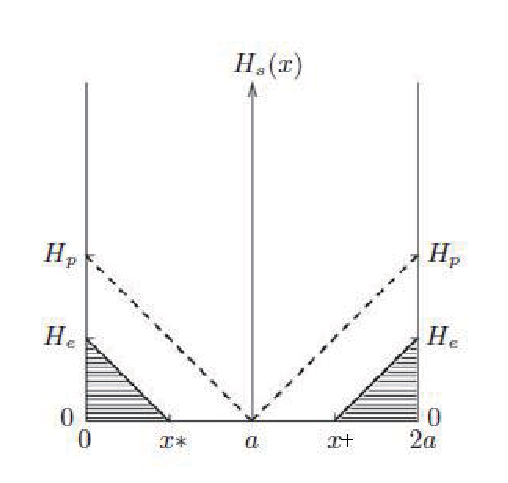
\includegraphics[scale=0.8]{chpt5/figs/fig5.1.eps}
  \caption{置于外磁场中的第II类超导体板}\label{fig:slabinfield}
\end{figure}
图\ref{fig:slabinfield}展示了第无限高($y$向)、无限深($z$向)、$2a$宽($x$向)第II类超导体板的。板此前未处于磁场中,外磁场$H_e$平行于板施加,将在板内产生$H_s(x)$。
根据安培定律$\nabla \times H = J=J_c$,我们可以得到超导体内的磁场$H_s(x)$:
\begin{subequations}
\begin{align}
 H_s(x)&=0, & \mbox{x*\le x \le x+ }  \\
H_s(x)&= H_e - J_c x, & \mbox{0\le x \le x* } \\
 H_s(x)&=H_e + J_c (x-2a), & \mbox{x+ \le x \le 2a}
\end{align}
\end{subequations}

注意到,$H_s(x)$的斜率等于$J_c$,当$J_c$大于0时(z向,朝向纸面外)大于0,$J_c$小于0时小于0。$x*$和$2a-x^+$给出磁场的穿透程度,表示为
\begin{equation}
  x*=\frac{H_e}{J_c}
\end{equation}

在$H_e=H_p\equiv J_c a$时,$x^*=x^+=a$,整个板处于临界态。$H_p$是所谓的穿透磁场,定义为
\begin{align*}
  H_p\equiv J_c a \tag{5.3b}
\end{align*}

板内的平均磁感应强度由下式给出:
\begin{subequations}
	\begin{align}
\~{B}_s&=\frac{\mu_0}{2a}\int_{0}^{2a} H_s(x)dx =\frac{\mu_0}{2a}\times <\mbox{图5.1中阴影面积}> \\
&=2\times \frac{\mu_0}{2a}\times \frac{H_e x^*}{2}=\frac{\mu_0 H_e^2}{2aJ_c}\\
&=\frac{\mu_0 H_e^2}{2H_p}
	\end{align}
\end{subequations}

根据定义$M=~{B}_s / \mu_0-H_e$,可得
\begin{equation}
  -M=H_e-\frac{H_e^2}{2H_p},(0\le H_e \le H_p)
\end{equation}

超导体是抗磁性的,-M是它的磁化强度。

随着外磁场的进一步增加,磁场将最终穿透整个板($H_e\ge H_p$),根据$~{B}_s=H_e-H_p/2$,有
\begin{equation}
  -M=\frac{1}{2}H_p=\frac{1}{2}J_c a, (H_e\ge H_p)
\end{equation}

图中的虚线磁化线对应$H_e=H_p$情况。
%5.2
\begin{figure}[htbp]
  \centering
 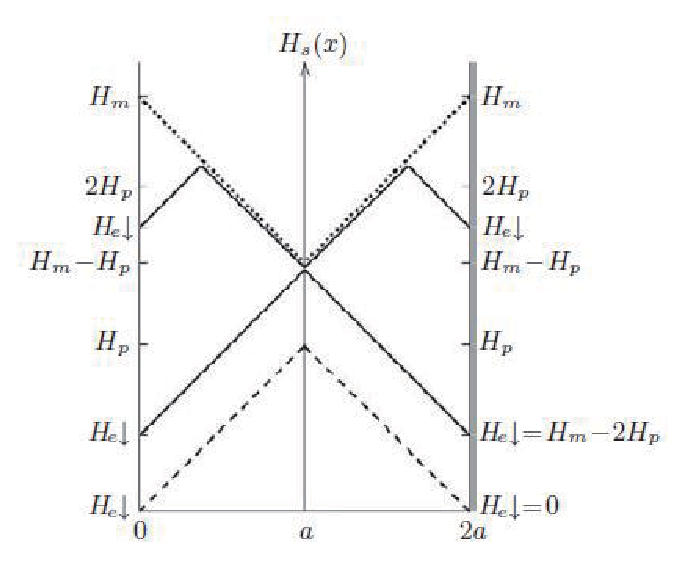
\includegraphics[scale=0.8]{chpt5/figs/fig5.2.eps}
  \caption{退场过程中的$H_s(x)$:$H_e\downarrow=H_m\rightarrow 0$}\label{fig:hreturn}
\end{figure}

图\ref{fig:hreturn}中的点线表示的是$H_s(x)$在$H_e=H_m>2H_p$时的情况。其中,$H_m$是外施磁场序列的最大值。

当$H_e$从$H_m$减至0的过程中,$H_s(x)$如图\ref{fig:hreturn}中的实线所示。当$H_e=H_m-2H_p$时,$-M$成为$-H_p /2$。
可以看到,外场从$H_m$到$H_e\downarrow=0$的退场过程中,$-M(H_e)$由下式给出

\begin{subequations}
\begin{align}
  -M(H_e) =&\frac{1}{2}H_p-(H_m-H_e)+\frac{(H_m-H_e)^2}{4H_p}\
\quad& (H_e\downarrow=H_m\rightarrow H_m-2H_p) \\
-M(H_e) =&-\frac{1}{2}H_p\quad &(H_e\downarrow=H_m-2H_p\rightarrow 0)
\end{align}
\end{subequations}


当外场施于“纯”板时,$-M$是$H_e$的二次函数。而在$H_e$退回0时,$-M(H_e)=-H_p /2$。“剩余”磁化如图\ref{fig:hreturn}中的虚划线所示。可知当置于外场中,
第II类超导体将会被磁化。剩余磁场不能通过外施磁场的方法去除。一种去除它的方法是加热超导体至临界温度$T_c$以上。
%5.3
\begin{figure}[htbp]
  \centering
 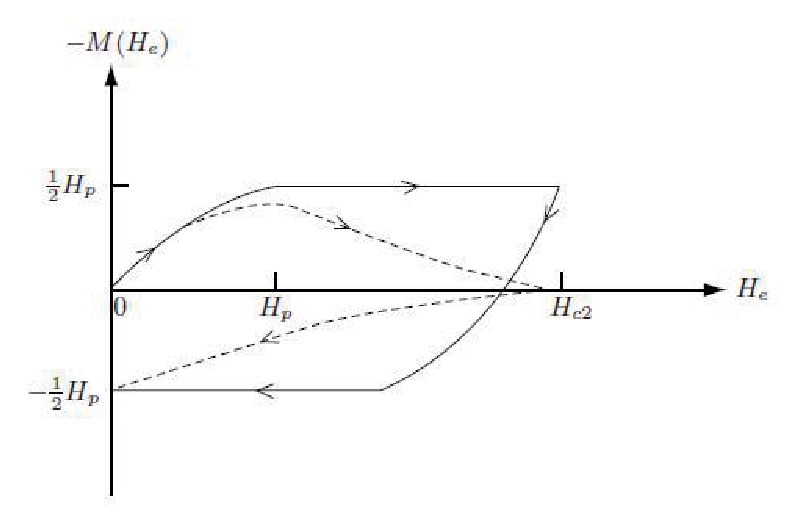
\includegraphics[scale=0.8]{chpt5/figs/fig5.3.eps}
  \caption{某硬超导体在外磁场($0\rightarrow H_{c2}\rightarrow 0$)下的磁化和磁场的关系。
  其中,实线表示$J_c=const$;虚线定性表示了电流随磁场下降的事实。}\label{fig:magvsh}
\end{figure}
图\ref{fig:magvsh}给出了完整的磁场从0增至$H_m=H_{c2}$又退回0的完整图像。其中,$H_{c2}$是超导体的上临界场。实线是基于由Bean的关于$J_c$不依赖磁场的假设
而导出的5.5-5.7式确定的。虚划线是对更接近实际情况的定性修正,反映了$J_c$随磁场衰减的事实,在$H_{c2}$时为0。注意到,磁化是有回滞的,在
$H_p<H_e<H_m-2H_p,\quad \Delta M=-M(H_e\uparrow)+M(H_e\downarrow)$范围内,磁场的幅值为$H_p=J_c a$。
于是,有时通过获得$J_e(H_e)$数据来做磁化的测量。
%5.4
\begin{figure}[htbp]
  \centering
 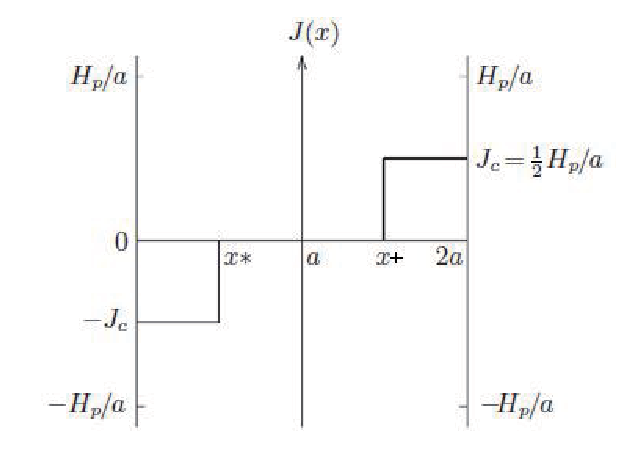
\includegraphics[scale=0.8]{chpt5/figs/fig5.4.eps}
  \caption{在图5.1给出的磁场$H_s(x)$下的$J(x)$}\label{fig:jtoh}
\end{figure}
图\ref{fig:jtoh}给出了在施加图\ref{fig:slabinfield}分布磁场下的板内电流分布。注意到$J_c=H_p /2a$。$y$向的单位长度净电流沿板的$z$向流动,由下式给出
\begin{equation}
  I=\int_{0}^{2a} J(x)dx=0
\end{equation}

\subsection{传输电流对励磁的效应}
当有传输电流$I_t$($y$向单位长度)在板中沿$+z$方向(流出纸面)时,我们看到在$x=2a$处磁场有一个$I_t/2$的增长,在$x=0$处有一个$I_t/2$的减少。

因为板内屏蔽电流是从每一个表面逐渐进入内部的,板内的场分布$H_s(x)$如图\ref{fig:hwithi}所示。图中的$x^*$和$x^+$由下式给出:
\begin{subequations}
	\begin{align}
  -\frac{1}{2}I_t + J_c x^* = 0 \\ 
J_c(x^*-2a)+\frac{1}{2}I_t = 0 \\ 
x^*=\frac{I_t}{2J_c}\quad \& \quad x^+ = 2a-\frac{I_t}{2J_c}
	\end{align}
\end{subequations}

\begin{figure}[htbp]
  \centering
 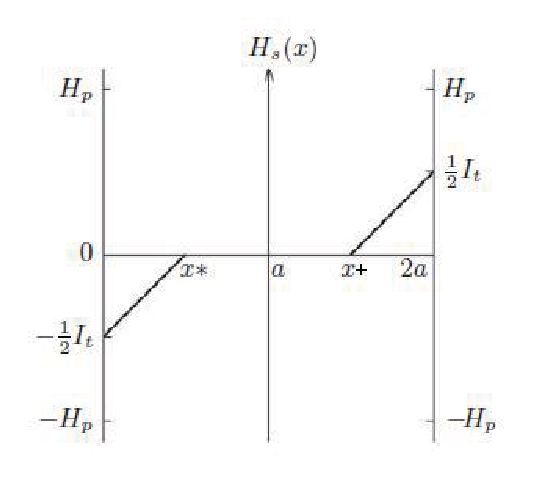
\includegraphics[scale=0.8]{chpt5/figs/fig5.5.eps}
  \caption{板内存在传输电流$I_t$时的磁场$H_s(x)$。}\label{fig:hwithi}
\end{figure}

图5.6给出了板内的电流分布$J(x)$。沿着板宽度方向积分,我们可以得到板内的净电流就是$I_t$:
\begin{subequations}
	\begin{align}
  I&=\int_{0}^{2a}J(x)dx=J_c x^*+J_c(2a-x^+)\\
  &=1/2 I_t +1/2 I_t=I_t
	\end{align}
\end{subequations}

\begin{figure}[htbp]
  \centering
 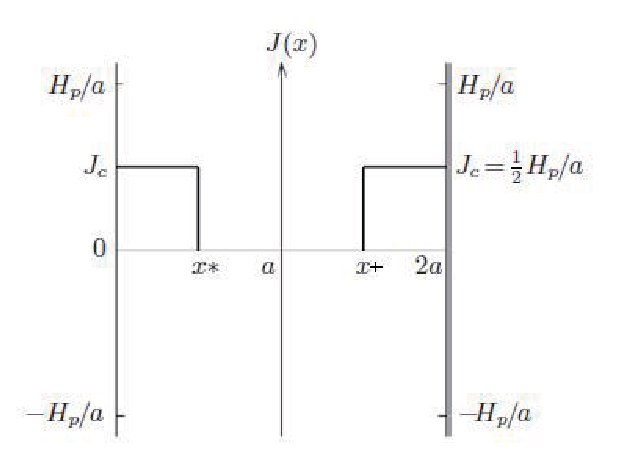
\includegraphics[scale=0.8]{chpt5/figs/fig5.6.eps}
  \caption{在图5.5给出的磁场$H_s(x)$下的$J(x)。$}\label{fig:jtoh5.5}
\end{figure}

也即,板内的净电流就是外施电流。注意到,若外磁场$H_e\vec{i_y}$在$I_t$通入后施加,基本不会改变电流的分布(图5.5和5.6);但若外磁场
先于电流施加,则会出现不同的$H_s(x)$和$J(x)$。讨论5.1中将详细研究传输电流对磁化的影响。

\section{测量技术}
这里我们描述最经常使用的测量磁化的技术。图5.7指示了本项技术的关键组件:1)初级探测线圈;2)次级探测线圈;3)平衡分圧计。
图中未画出但也同等重要的是积分器,它将桥路输出电压$V_bg$转换为直接正比于$M(H_e)$的电压信号。测试样品置于初级探测线圈内,。
当初级探测线圈和次级探测线圈置于在两个线圈所占的空间内基本均匀的时变外磁场$H_e(t)$中,各查找线圈的端子上将出现感应
电压$V_{pc}(t)$和$V_{sc}(t)$:
\begin{subequations}
	\begin{align}
  V_{pt}(t) &=\mu_0 N_{pc} A_{pc}\left[\frac{dM}{dt}+(\frac{d\~{H}_e}{dt})_{pc}\right] \\ 
V_{sc}(t) &= \mu_0 N_{sc} A_{sc}\left( \frac{d\~{H}_e}{dt}\right)_{sc}
	\end{align}
\end{subequations}
下标pc和sc分别表示初级线圈(primary coil)和次级线圈(second coil)。N是各线圈的匝数。A是耦合$H_e(t)$的每一匝线圈的有限面积。
$\~{H}_e$是磁场在各线圈内的空间平均值。

桥输出电压$V_bg$由下式给出:
\begin{equation}
  V_{bg}(t)=(k-1)V_{pt}(t)+kV_{sc}(t)
\end{equation}

其中,k是一个介于0-1的常数,表示分压计在初级线圈侧的分压系数(图5.7)。联立上两式,可得
\begin{align}
  V_{bg}(t)=&(k-1)\mu_0 N_{pc}A_{pc}\frac{dM}{dt}\\
  &+(k-1)\mu_0 N_{pc}A_{pc}(\frac{d\~{H}_e}{dt})_{pc}+k\mu_0 N_{sc}A_{sc}(\frac{d\~{H}_e}{dt})_{sc}
\end{align}

%%图5.7
\begin{figure}[htbp]
  \centering
 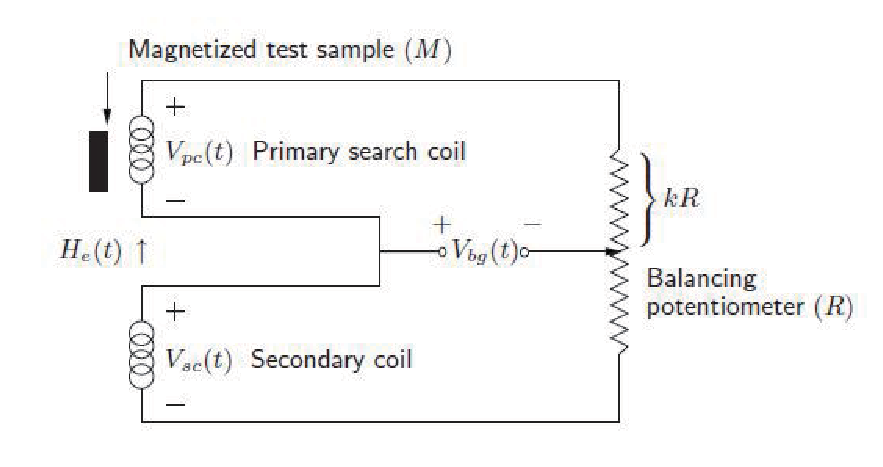
\includegraphics[scale=0.8]{chpt5/figs/fig5.7.eps}
  \caption{磁化测量原理图}\label{fig:magmeasure}
\end{figure}

通过调节分压系数k可以满足以下条件,令$V_{bg}(t)$正比于$dM/dt$:
\begin{subequations}
	\begin{align}
  (k-1)\mu_0 N_{pc}A_{pc}(\frac{d\~{H}_e}{dt})_{pc}+k\mu_0 N_{sc}A_{sc}(\frac{d\~{H}_e}{dt})_{sc}=0 \\ 
V_{bg}(t)=(k-1)\mu_0 N_{pc}A_{pc}\frac{dM}{dt}
	\end{align}
\end{subequations}

尽管实际上上式第一式所给的归零条件在很大范围内不是总能满足,但是第二式对多数情况都是很好的近似。
一般,$k$接近0.5。$V_bg{t}$馈入一个积分器,其输出正比于$M$。特别的,如果样品是“纯”的($M=0$),磁场
$H_e(t)$从0($t=0$)增($\uparrow$)至$H_e$($t=t_1$)时,我们有
\begin{equation}
  V_{mz}(H_e\uparrow)=\frac{1}{\tau_{it}}\int_{0}^{t_1}V_bg(t)dt=\frac{(k-1)\mu_0 N_{pc}A_{pc}}{\tau_{it}}M(H_e)
\end{equation}
式中,$\tau_{it}$是有效积分常数。如果$H_e>H_p$,此时有$M(H_e)=-H_p / 2=-J_c a / 2$,则上式简化为
\begin{equation}
    V_{mz}(H_e\uparrow>H_p)=-f_m \frac{(k-1)\mu_0 N_{pc}A_{pc}}{\tau_{it}}\left(\frac{J_c a}{2}\right)
\end{equation}

因数$f_m$是磁性材料体积与样品总体积之比。之所以需要这个因数是因为待磁化测试的样品一般不全是由磁性材料组成。
比如多丝(层)导体,样品除了超导丝(层)外,还存在基底金属和其他非磁性材料。如果外场按$0\rightarrow H_m>H_p\rightarrow H_e\downarrow <H_m-2H_p$顺序,
我们有:
\begin{align*}
    V_{mz}(H_e\downarrow<H_m-2H_p)=-f_m \frac{(k-1)\mu_0 N_{pc}A_{pc}}{\tau_{it}}(\frac{J_c a}{2}) \tag{5.16b}
\end{align*}

于是,$\Delta V_{mz}=V_{mz}(H_e>H_p)-V_{mz}(H_e\downarrow<H_m-2H_p)$正比于在$H_e$处磁化曲线的“宽度”:
\begin{align*}
    \Delta V_{mz}=-f_m \frac{(k-1)\mu_0 N_{pc}A_{pc}}{\tau_{it}} J_c a \tag{5.16c}
\end{align*}

上式我们看出,$\Delta V_{mz}$是直接正比于$J_c$和$a$的。
%%图5.8
\begin{figure}[htbp]
  \centering
 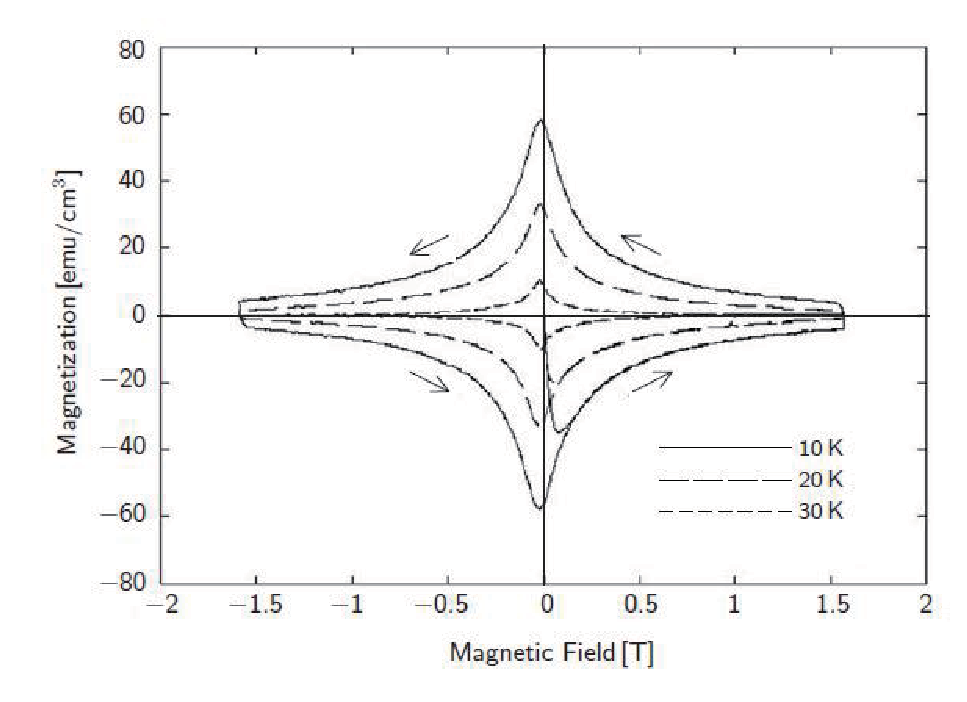
\includegraphics[scale=0.7]{chpt5/figs/fig5.8.eps}
  \caption{$MgB_2$在$10K,20K,30K$三种温度下的磁化和磁场关系}\label{fig:magvfield}
\end{figure}

图5.8给出的是$MgB_2$在10K,20K,30K时,磁场按$0\rightarrow 1.7T\rightarrow 0 \rightarrow -1.7T\rightarrow 0$完整施加时的磁化与磁场的关系。注意到,
和图5.3不同,本图中还有$+M(H_e)$。因为凸显在$x$轴上(磁场)并不偏斜,我们可以认为本测试中初次、二次线圈已得到很好的平衡。

磁化的回滞表明,$MgB_2$是第II类超导体,它的抗磁性在每一个图线的第一部分(磁场从0增至1.7T时)明显可见。

从Bean模型可知,$H_p=J_c a$,即磁化直接正比于$J_c$。
然而,实际上$J_c$不仅是磁场还是温度的减函数。图5.8中明显可见对$J_c$和$T$的依赖。
图中的$M$的单位是$emu/cm^3$,不是SI单位。

\section{专题}
\subsection{讨论5.1:有传输电流时的磁化}
正如本书最初所述,在传输电流存在条件下的磁化依赖于外场和传输电流施加的顺序。
这里我们考虑三种情况:A) 先加磁场后加传输电流; B) 先通电流后加磁场;C) 磁场和电流交替改变。

\textbf{A.  先加磁场后加传输电流}

图5.9给出了厚度为$2a$的Bean板在施加如下特定磁场-电流序列后内部磁场$H_s(x)$的特征。
\begin{enumerate}
	\item 起始,$H_{s1}(x)$,有$H_e=2.5H_p$,无传输电流——点线。
	\item 接下来,$H_{s2}(x)$,通过传输电流$I_t=J_c=I_c/2$后,施加恒定外场——实线。其中,$J_c a=H_p$。
	\item 最后,$H_{s3}(x)$,传输电流进一步增加到$2J_c a=I_c$后,磁场$H_e =2.5 H_p$,最终$H_{s3}(0)=1.5 H_p$
	以及$H_{s3}(2a)=3.5H_p$——虚线。
\end{enumerate}

$H_{s1}(x)$和$H_{s3}(x)$是很直接的。$H_{s2}(x)$由三个分段函数$H_{s2_1}(x),H_{s2_2}(x),H_{s2_3}(x)$组成:
\begin{align*}% page321 第1个
H_{s2_{1}}(x)&=2H_{p}+J_{c}x=2J_{c}a+J_{c}x\qquad&(0\leq x\leq x*)\\
H_{s2_{2}}(x)&=2.5H_{p}-J_{c}x=2.5J_{c}a-J_{c}x\quad&(x*\leq x\leq x+)\\
H_{s2_{3}}(s)&=H_{p}+J_{c}x=J_{c}a+J_{c}x\qquad&(x+\leq x\leq 2a)
\end{align*}
式中,$x*$和$x+$由$H_{s1}(x)$和$H_{s2}(x)$的两个拐点给出。也即,$H_{s1}(x*)=H_{s2_1}(x*)$,
$H_{s1}(x+)=H_{s2_3}(x+)$:$x*=0.25a$,$x+=0.75a$。
\begin{figure}[htbp]
	\centering
	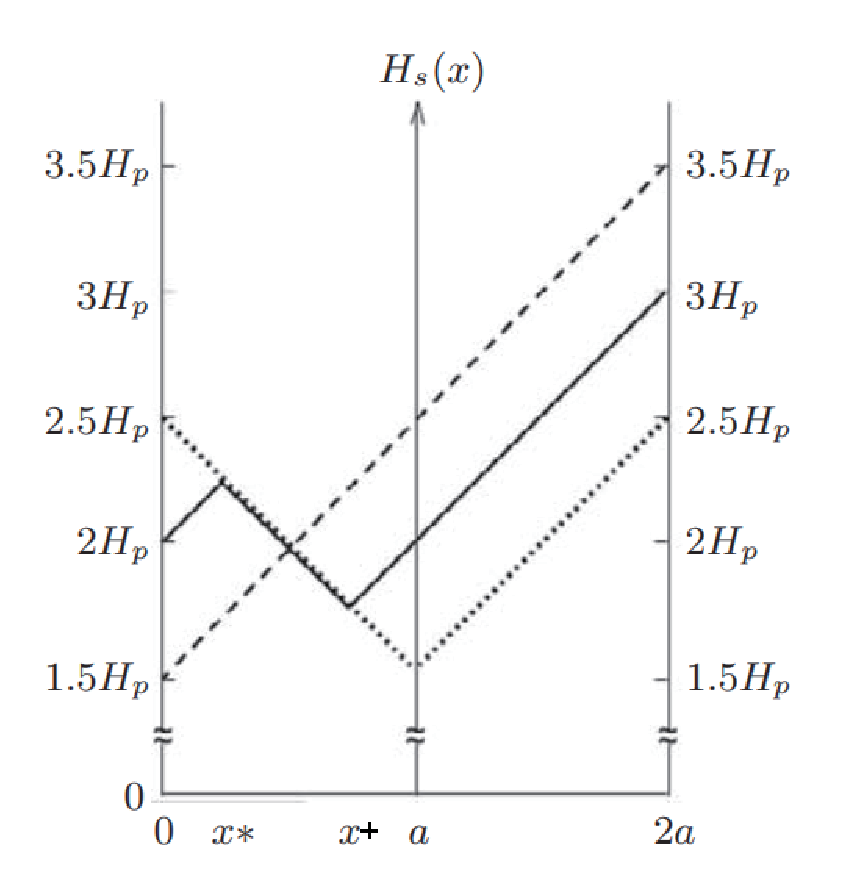
\includegraphics[scale=0.6]{chpt5/figs/fig5.9.eps}
	\caption{在$H_e=2.5H_p$下的磁场特征。首先,$I_t$=0(点线),然后$I_t=J_c a=I_c/2$(实线),最后$I_t=2J_c a=I_c$(虚线)。}
\end{figure}

图5.10给出了在$I_t$存在时$H_s(x)$作为$H_{s2_1}(x)$,$H_{s2_2}(x)$和$H_{s2_3}(x)$的分段函数(实线)的一般情况。
如5.2.2所述,$I_t$($z$轴)是$y$轴单位长度的传输电流。
这里,我们定义一个无量纲传输电流$i\equiv I_t/I_c$,其中$I_c=2aJ_c$。
$\int H_s(x)$积分时,图5.10中的板分成三个面积$A_1,A_2,A_3$,分界线即图中的竖直虚线。
注意到,$I_t=i I_c=2iaJ_c=2iH_p$。

面积$A_1(0\le x\le x^*)$中的磁场$H_{s2_1}(x)$、面积$A_2(x^*\le x\le x^+)$中的磁场$H_{s2_2}(x)$、
面积$A_3(x^+\le x\le 2a)$中的磁场$H_{s2_3}(x)$分别为:
\begin{align*}
H_{s2_{1}}(x)&=(H_{e}-\frac{1}{2}I_{t})+J_{c}x\qquad&(0\leq x\leq x*)\\
H_{s2_{2}}(x)&=H_{e}-J_{c}x\qquad&(x*\leq x\leq x+)\\
H_{s2_{s}}(x)&=(H_{e}+\frac{1}{2}I_{t})+J_{c}(x-2a)\qquad&(x+\leq x\leq2a)
\end{align*}

我们解出$x^*$和$x^+$,确定$H_{s2_2}(x^*)$和$H_{s2_2}(x^+)$:
\begin{align*}
&H_{{s}2_{1}}(x*)=H_{s2_{2}}(x*)\\
&H_{e}-H_{p}i+J_{c}x*=H_{e}J_{c}x*\Rightarrow x*=\frac{H_{p}}{2J_{c}}i=\frac{1}{2}ai\\
&H_{s2_{2}}(x*)=H_{e}-\frac{1}{2}aJ_{c}i=H_{e}-\frac{1}{2}H_{p}i
\end{align*}
以及
\begin{align*}
H_{s2_{2}}(x+)&=H_{s2_{3}}(x+)\\
H_{e}-J_{c}x+&=H_{e}+H_{p}i+J_{c}(x^{+}-2a)\Rightarrow x^{+}=a(1-\frac{1}{2}i)\\
H_{s2_{2}}(x+)&=H_{e}-H_{p}+\frac{1}{2}H_{p}i
\end{align*}

\begin{figure}[htbp]
	\centering
	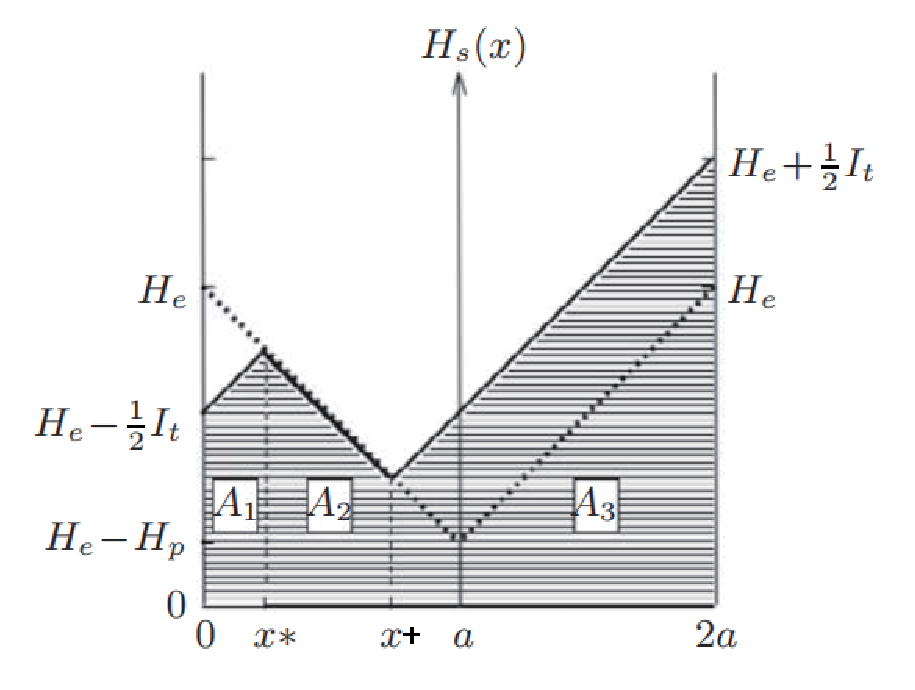
\includegraphics[scale=0.6]{chpt5/figs/fig5.10.eps}
	\caption{用于励磁计算的有传输电流(实线)的磁场的特征。竖直点线分开三个区域:$A_1, A_2$和$A_3$。}
\end{figure}

$M$正比于如图5.10所示的``阴影面积``大小,是三个部分面积$A_1, A2$及$A_3$之和。

各梯形的面积为它的``底边$\times$(高1+高2)/2``。
\begin{align*}% page323 第1个
A_{1}&=\frac{1}{2}x*[H_{s1}(0)+H_{s2}(x*)]=\frac{1}{4}ai[(H_{e}-H_{p}i)+(H_{e}-\frac{1}{2}H_{p}i)]\\
&=\frac{1}{4}ai(2H_{e}-\frac{3}{2}H_{p}i)  \\
&=a(\frac{1}{2}H_{e}i-\frac{3}{8}H_{P}i^{2})\\
A_{2}&=\frac{1}{2}(x^{+}-x*)[H_{s2}(x*)+H_{s2}(x^{+})]\\
&=\frac{1}{2}(a-ai)(H_{e}-\frac{1}{2}H_{p}i+H_{e}-H_{p}+\frac{1}{2}H_{p}i)\\
&=\frac{1}{2}a(-i)(2H_{e}-H_{p})\\
&=a(H_{e}-H_{e}i-\frac{1}{2}H_{p}+\frac{1}{2}H_{p}i)\\
A_{3}&=\frac{1}{2}(2a-x+)[H_{s2}(x+)+H_{s3}(2a)]\\
&=\frac{1}{2}(a+\frac{1}{2}ai)(H_{e}-H_{p}+\frac{1}{2}H_{p}i+H_{e}+H_{P}i)\\
&=a(1+\frac{1}{2}i)(H_{e}-\frac{1}{2}H_{p}+\frac{3}{4}H_{p}i)\\
&=a(H_{e}+\frac{1}{2}H_{e}i-\frac{1}{2}H_{p}-\frac{1}{4}H_{p}i+\frac{3}{4}H_{p}i+\frac{3}{8}H_{p}i^{2})
\end{align*}

组合这三个面积,我们可以计算出阴影面积:
\begin{align*}% page323 第4个
\mbox{阴影面积}=&A_{1}+A_{2}+A_{3}\\
=&a(\frac{1}{2}H_{e}i-\frac{3}{8}H_{p}i^{2}+H_{e}-H_{e}i-\frac{1}{2}H_{p}+\frac{1}{2}H_{p}i\\
&+H_{e}+\frac{1}{2}H_{e}i-\frac{1}{2}H_{p}-\frac{1}{4}H_{P}i+\frac{3}{4}H_{P}i+\frac{3}{8}H_{p}i^{2})\\
=&a(2H_{e}-H_{p}+H_{p}i)
\end{align*}

一旦阴影面积已知,$M$可快速算出:
\begin{subequations}
	\begin{align}
-M(i)&=H_{e}-\frac{1}{2a}\mbox{阴影面积}\\\notag
&=H_{e}-H_{e}+\frac{1}{2}H_{p}-\frac{1}{2}H_{p}i\\\notag
&=\frac{1}{2}H_{p}(1-i)\\
&=-M(0)f_{1}(i)
	\end{align}
\end{subequations}
\begin{align*}% page323 第4个

\end{align*}
式中,$f_1(i) = 1 − i$。$−M(i)$线性随$i$减小,当$i=1$时为零。 

\textbf{B. 先通电流后加磁场}

这里向板加外部磁场和传输电流顺序是反过来的。
特别的,传输电流$J_c=(I_c/2)\vec{i_z}$(纸面向外)是在板“无染”时通入的。
而后,保持$I_t$恒定,在$+y$向施加幅值为$2H_p$的外场。

在图5.11中,点线表示传输电流$J_c a(=H_p/2)$施加之后,但$H_e(=2H_p)$施加之前的$H_s(x)$;
实线表示$H_e(=2H_p)$施加之后的$H_s(x)$。
两种情况下,板中的净电流都是$J_c a$。

开始,$H_e=0$:
\begin{align*}% page324 第1个
I_{t}=\int_{0}^{2a}J(x)dx=J_{c}(0.5)+J_{c}(2a-1.5a)=J_{c}a
\end{align*}

接下来,$H_e=2H_p$:
\begin{align*}% page324 第2个
I_{t}=\int_{0}^{2a}J(x)dx=-J_{c}(0.5a)+J_{c}(2a-0.5a)=J_{c}a
\end{align*}

为了确定任意电流($I<I_c$)下板内的磁化一般情况,
我们首先找到$x^*$(图5.12),它可由区域I内($0\le x\le x^*$)的实线$H_{s1}(x)$
和区域II内$(x^*\le x\le 2a)$的$H_{s2}(x)$确定。
\begin{align*}
H_{s1}(x)&=(H_{e}-H_{p}i)-J_{c}x\qquad(0\leq x \leq x*)\\
H_{s2}(x)&=(H_{e}+H_{p}i)+J_{c}(x-2a)\quad(x*\leq x \le  2a)
\end{align*}
因为$H_{s1}(x*)=H_{s2}(x*)$,我们从上式解出$x*$:
\begin{align*}% page324 第5个
x*=a-ai=a(1-i)
\end{align*}

\begin{figure}[htbp]
	\centering
	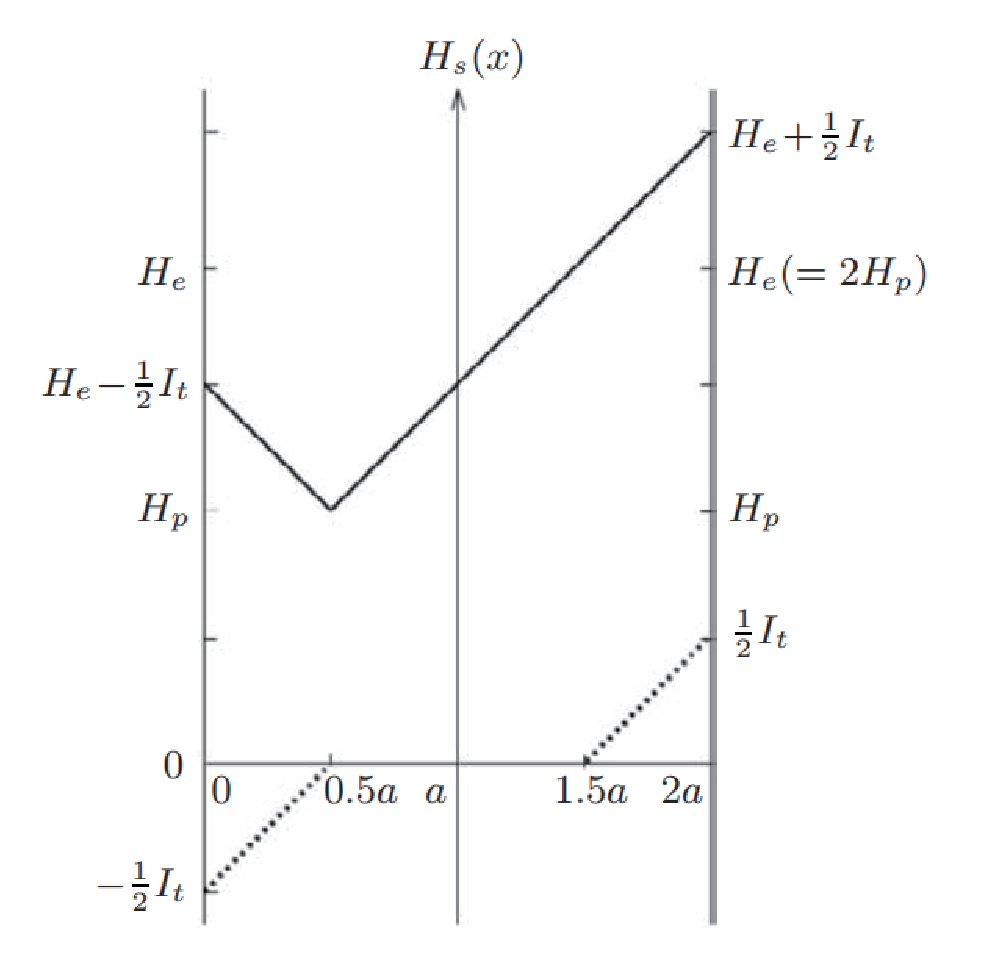
\includegraphics[scale=0.5]{chpt5/figs/fig5.11.eps}
	\caption{磁场特征,点线表示仅有电流,实现表示有磁场和电流。}
\end{figure}

确定了$x*$之后,我们可以计算$H_{s1}(x∗)$:
\begin{align*}% page325 第1个
H_{s1}(x*)=H_{e}-H_{p}i-J_{c}a(1-i)=J_{e}-H_{p}
\end{align*}

接下来我们可以计算阴影下的面积,即如图5.12中所示的由竖直线分开的$A_1$和$A_2$两部分之和:
\begin{align*}% page325 第2个
A_{1}&=\frac{1}{2}a(1-i)(H_{e}-H_{p}i+H_{e}-H_{p}\\
&=a(1-i)(H_{e}\frac{1}{2}H_{p}-\frac{1}{2}H_{p}i)\\
&=a(H_{e}-H_{e}i\frac{1}{2}H_{p}+\frac{1}{2}H_{p}i^{2})\\
A_{2}&=\frac{1}{2}(2a-a+ai)(H_{e}+H_{p}i+H_{e}-H_{P})\\
&=a(1+i)(H_E-\frac{1}{2}H_{p}+\frac{1}{2}H_{p}i)\\
&=a(H_{e}+H_{e}-\frac{1}{2}H_{p}+\frac{1}{2}H_{p}i^{2})\\
\mbox{阴影面积}&=A_{1}+A_{2}\\
&=a(2H_{e}-H_{p}+H_{p}i^{2})
\end{align*}

计算了阴影面积后,我们有$M$:
\begin{subequations}
	\begin{align}
-M(i)&=H_{e}-\frac{1}{2}(2H_{e}-H_{p}+H_{p}i^{2}\\\notag
&=\frac{1}{2}H_{p}(1-i^{2})\\
&=-M(0)f_{2}(i)
	\end{align}
\end{subequations}
式中,$f_2(i) = 1 − i^2$。励磁时电流$i$的二次函数。

\begin{figure}[htbp]
	\centering
	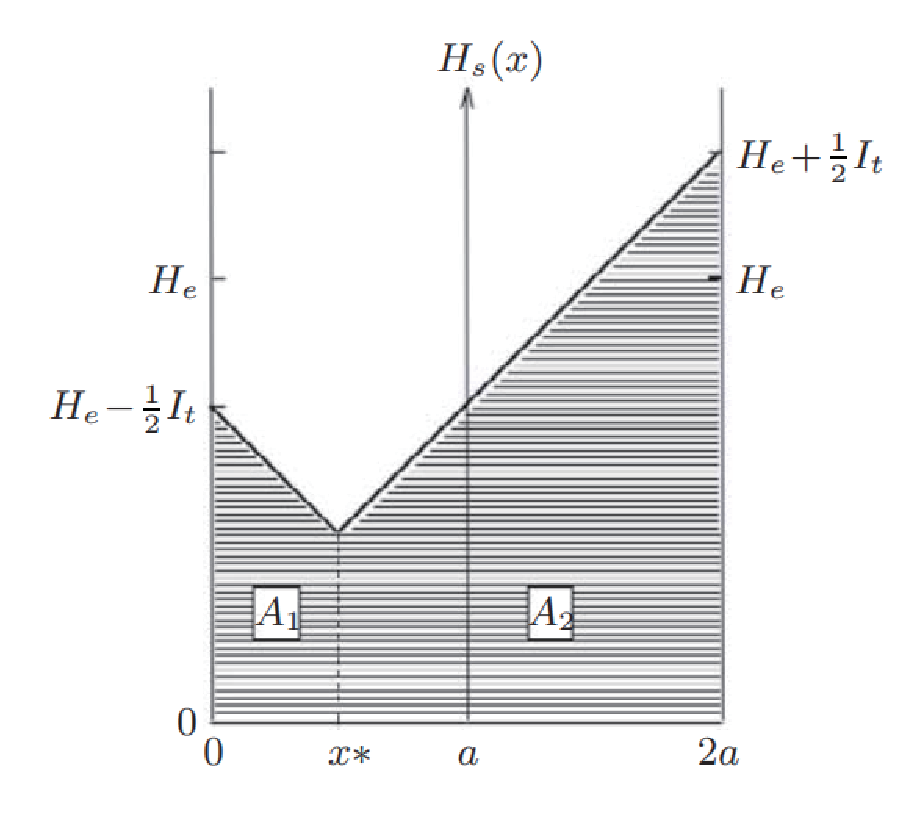
\includegraphics[scale=0.5]{chpt5/figs/fig5.12.eps}
	\caption{计算同时有传输电流和磁场时的磁化的场特性。竖直点线分出两个区域$A_1$和$A_2$。}
\end{figure}


\textbf{C. 先加磁场,后改变电流}

最后,我们可以考虑按照以下序列施加磁场和传输电流时的$H_s(x)$和$−M(i)$。

\begin{enumerate}
	\item 从“无染”板开始,$I_t$为零,在$+y$向施加外场$H_e=2H_p$。
	\item 在$H_e$保持$2H_p$时,向板内通入$z$向(纸面向外)传输电流$I_t=2H_p i$,其中$i=I_t/I_c$。
	\item 维持$H_e=2H_p$,将$I_t$减至零。
	\item $I_t$反向,向板内通入$-z$向(纸面向内)传输电流$|2H_p i|$。
	\item $I_t$再次减至零;$H_e$保持$2H_p$不变。
\end{enumerate}

图5.13给出了第5步之后的磁场$H_s(x)$特性,它由五段实线组成,第2段和第3段对计算$M(i)$有用,
分别为:
\begin{align*}
H_{s2}(x)&=H_{e}+H_{p}i-J_{c}x\qquad(x*\leq x\leq a)\\
H_{s3}(x)&=H_{e}+H_{p}i+J_{c}(x-2a)\quad(a\leq x\leq a^{+})
\end{align*}
式中,$x∗$和$x$可由$H_{s2}(x∗)=H_{s3}(x)=H_e$解出。于是:
\begin{align*}
H_{s2}(x*)&=H_{e}\Rightarrow H_{e}+H_{p}i-J_{c}x*\\
x*&=\frac{H_{p}i}{J_{c}}=ai\\
H_{s3}(x+)&=H_{e}\Rightarrow H_{e}+H_{P}i+J_{c}(x^{+}-2a)\\
x^{+}&=2a-\frac{H_{p}}{J_{c}}i=2a-ai
\end{align*}

\begin{figure}[htbp]
	\centering
	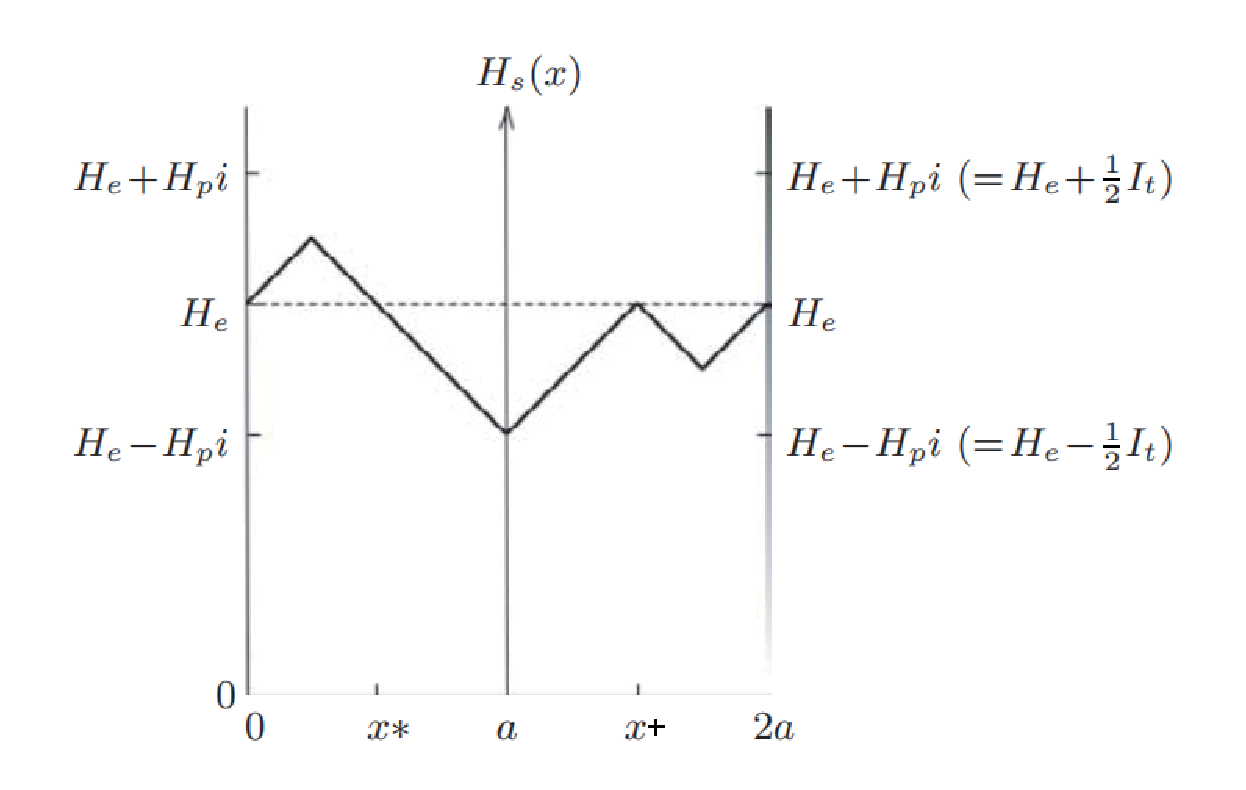
\includegraphics[scale=0.5]{chpt5/figs/fig5.13.eps}
	\caption{第五步之后的磁场特征。}
\end{figure}

磁化由图5.14给出的合适的面积计算得到。其中,板从左到右被分为4个白色面积,
分别记为$A_1$(长方形)、$A_2$(梯形)、$A_3$(梯形)和$A_4$(长方形-三角形)。
图中,“底”和“高”分别为:
\begin{align*}
\mbox{底}&=x+-x*=(2a-ai)-ai=(a(1-i)\\
\mbox{高}&=H_{e}-H_{s2}(a)=H_{e}-(H_{e}+H_{p}i-J_{c}a)\\
&=J_{c}a-J_{p}i=H_{p}(1-i)
\end{align*}

图5.14中的两个填充“点”的面积大小相等但符号相反,因此
计算积分的时候可以抵消。所以,
$A_1$、$A_2$、$A_3$和$A_4$面积之和为:
\begin{align*}
\sum_{j=1}^{4}A_{j}&=2aH_{e}-\mbox{叉填充区域}\\
\mbox{叉填充区域}&=\frac{1}{2}(\mbox{底})\times(\mbox{高})\\
\sum_{j=1}^{4}A_{j}&=2aH_{e}-\frac{1}{2}2a(1-i)H_{p}(1-i)\\
&=2aH_{e}-aH_{p}(1-i)^{2}
\end{align*}

于是,磁化$−M(i)$可如下给出:
\begin{align*}% page327 第6个
-M(i)=&H_{e}-\frac{1}{2a}[2aH_{e}-a \grave{}H_{p}(1-i)^{2}]\\
=&\frac{1}{2}H_{p}(1-i)^{2}\\\notag
\end{align*}
\begin{subequations}
	\begin{align}% page327 第6个
	-M(i)=&-M(0)(1-i)^{2}\\
	=&-M(0)f_{3}(i)
	\end{align}
\end{subequations}
式中,$f_3(i) = (1 − i)^2$。

\begin{figure}[htbp]
	\centering
	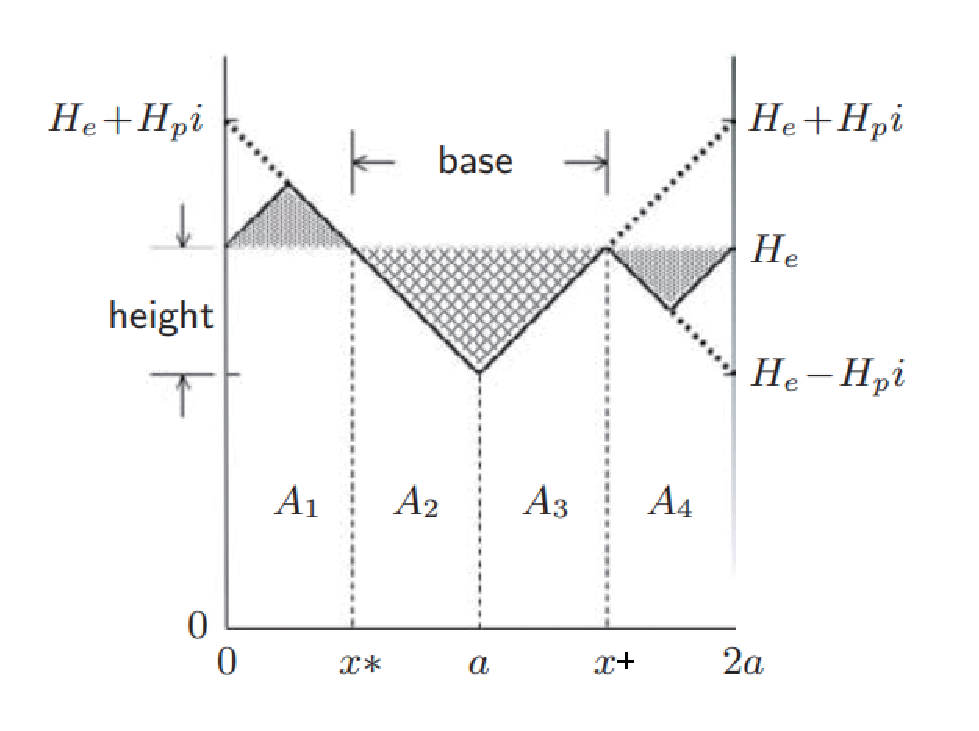
\includegraphics[scale=0.5]{chpt5/figs/fig5.14.eps}
	\caption{用以计算励磁的第五步之后的磁场特征。}
\end{figure}

\begin{figure}[htbp]
	\centering
	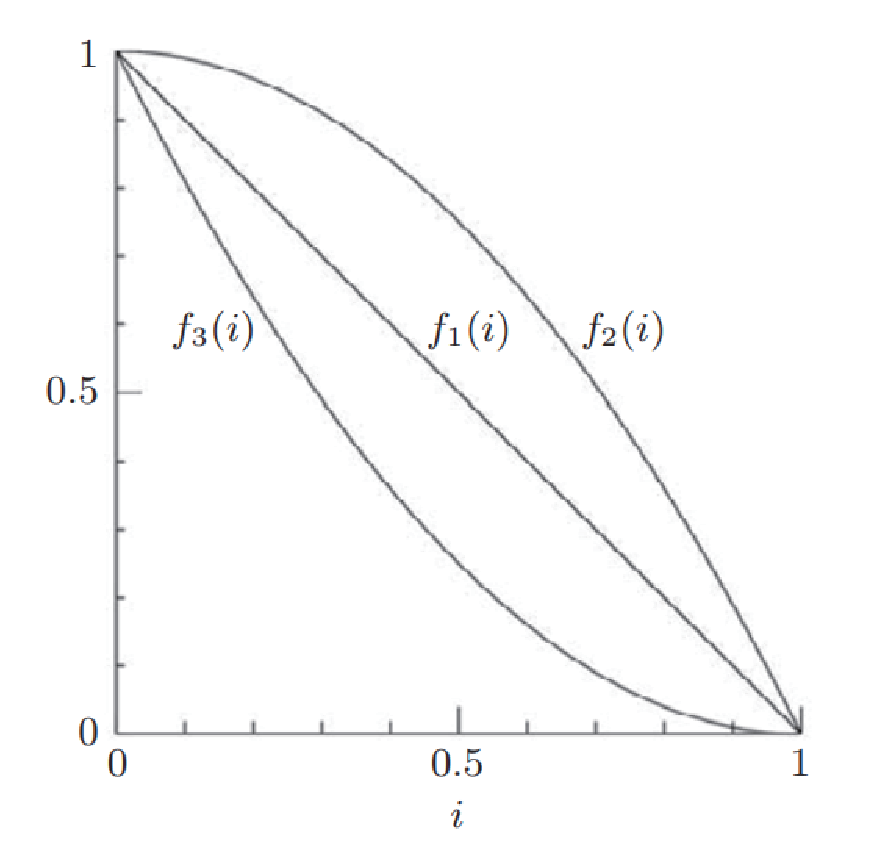
\includegraphics[scale=0.5]{chpt5/figs/fig5.15.eps}
	\caption{讨论5.1研究的三种归一化励磁 vs. 归一化电流关系。}
\end{figure}

\textbf{磁化函数---总结}

图5.15给出三个归一化磁化函数$f_1(i), f_2(i)$和$f_3(i)$。其中,$i = I_t/I_c$。
很有意思的是,传输电流和外部磁场施加的不同顺序影响$M(i)$。
这些$f(i)$函数已得到试验验证[5.3, 5.4],故而Bean模型在提出之后很快就被人们接受了。


\subsection{讨论5.2:SQUID用于磁化测量}
SQUID (Superconducting Quantum Interference Device,超导量子干涉仪)是基于Josephson效应的一种电子
器件,可以极高的分辨率——单个磁通量子,幅值$2.0\times 10^{−15}\ \mathrm{Wb(Tm^2)}$——来测量磁场的变化。

一个典型的SQUID磁化测量装置的测试样品处于恒温,置于均匀磁场中。
测试样品在均匀场中前后移动;每一个周期内它切过分别位于测试样品两端的两个测试线圈。
每一个测试线圈中感应的电流产生的磁场由SQUID检测,反过来,这就是测试样品的磁化。
因为SQUID在低磁场环境下运行的最好( 不高于100 oersted或0.01 T),
通常要将之与测试样品的高场环境屏蔽。


\subsection{讨论5.3:“Bean细丝”中的磁化}
\subsubsection{第一部分:磁场平行于细丝轴}
我们使用Bean推导它的磁化表达式相同的假设,将一根直径$d_f$、无限长的超导细丝,
置于平行于细丝轴(z)d的外磁场$H_e\vec{i_z}$中。
对于置于$H_e\vec{i_z}$中的无限长细丝,应用Ampere定律:
\begin{equation}% page329 第1个
\frac{dH_{z}}{dr}\vec{\imath}_{\theta}=-J_{c}\vec{\imath}_{\theta}
\end{equation}
方程5.20表明,细丝内的轴向(z)磁场$H_s(r)$是r的线性函数,斜率为$J_c$。

\textbf{A. 初始态}

在$H_e \le H_p$时,($H_p$是临界态磁场),细丝内的磁场$H_s(r)$从$r=0$到$r*=(d_f/2-H_e/J_c)$之间为零,
并从$r*$到$d_f/2$随$J_c r$变化: 
\begin{equation}% page329 第2个
H_{s}(r)=H_{e}\frac{r-r*}{\frac{d_{f}}{2}-r*}
\end{equation}

我们注意到在$H_e=H_p$时,$r*=0$。其中,$H_p$是临界态磁场。
\begin{equation}% page329 第3个
H_{p}=\frac{1}{2}J_{c}d_{f}
\end{equation}

使用方程5.4那里类似的步骤,我们可以计算细丝内的平均磁感应$\tilde{B}_s$:
\begin{align}% page329 第4个
\tilde{B_{s}}&=\frac{4\mu_{o}}{\pi d_{f}^{2}}\int_{r*}^{\frac{d_{f}}{2}}H_{e}\frac{r-r*}{\frac{d_{f}}{2}-r*}(2\pi r)dr\\
&=\frac{8\mu_{o}H_{e}}{d_{f}^{2}(\frac{d_{f}}{2}-r*)}(\frac{1}{24}d_{f}^{3}-\frac{1}{8}d_{f}^{2}r*+\frac{1}{6}r*^{3})
\end{align}

和板的情况不同,那里积分可以$H_s(x)$几何的形式得到。这里,“面积”积分必须
用数学的方法进行。向5.23中代入$r*=(d_f/2−H_e/J_c)$,并注意到$H_p=J_cd_f/2$,我们有:
\begin{equation}%page329 第5个
\frac{\tilde{B}_{s}}{\mu_{o}}=\frac{2H^{2}_{e}}{d_{f}J_{c}}-\frac{4H^{3}_{e}}{3(d_{f}J_{c})^{2}}=\\frac{H^{2}_{e}}{H_{P}}-\frac{H_{e}^{3}}{3H^{2}_{p}}
\end{equation}

根据$M=\~{B}_s/\mu_{0}-H_e$,我们有:
\begin{equation}%page329 第6个
-M=H_{e}-\frac{H^{2}_{e}}{H_{P}}+\frac{H^{3}_{e}}{3H^{2}_{p}}\quad(0\leq H_{e}\leq H_{P})
\end{equation}

可见,方程5.25与板情况的方程5.5类似,但也存在明显的不同。

\textbf{B. 临界态及以上}

在$H_e\ge H_p$时,细丝为临界态,其磁化是定值,可由方程5.25在$H_e=H_p$时得到:
\begin{equation}%page329 第7个
-M=\frac{1}{3}H_{p}=\frac{1}{3}(\frac{J_{c}d_{f}}{2})\quad(H_{e}\geq H_{p})
\end{equation}

细丝的“磁化因子”是$1/3$;板是$1/2$ (方程5.6)。

\subsubsection{第二部分:磁场垂直于细丝轴}
当外施场垂直于直径为$d_f$的细丝的轴,细丝内部的电流分布在$H_e\le H_p$时较为复杂;
$H_e\ge H_p$时,在$+z$向感应出的总电流为$J_c \pi d^2 f/8$,$-z$向感应电流幅值相等
图5.16给出几种电流分布:a) $2a$的Bean板;b) 直径为$d_f$的细丝。

我们可以通过对单位体积的磁矩$\mathbf{m_A}$得到磁化强度$M$。
这里,我们宽度为$2a$的Bean板和直径为$d_f$的细丝的临界态磁化表达式。

\textbf{A. Bean板}

对处于临界态的Bean板,$z$向和$y$向的单位长度磁矩$\mathbf{m_A}$由图5.16a中的$J_c(x)$可知,为:
\begin{equation}%page330 第1个
m_{A}=\int_{0}^{a}2xJ_{c}(x)dx=J_{c}a^{2}
\end{equation}
$z$向和$y$向单位长度的体积为$2a$。于是:
\begin{align*}%page330 第2个
M=\frac{m_{A}}{2a}=\frac{1}{2}J_{c}a \tag{5.27b}
\end{align*}
方程5.27b给出的$M$除了符号,和方程5.6一致。

\textbf{B. 细丝}

对直径为$d_f$的细丝,$z$向单位长度的磁矩$\mathbf{m_A}$由图5.16b的$J_c(x,y)$可知,为:
\begin{equation}%page330 第3个
m_{A}=\int_{-\frac{d_{f}}{2}}^{\frac{d_{f}}{2}}2xJ_{c}(x,y)dxdy=\frac{1}{6}J_{c}d_{f}^{2}
\end{equation}
$z$向单位长度导体体积为$\pi d_f^2/4$。于是:
\begin{subequations}
	\begin{align}
M&=\frac{\mathbf{4m_{A}}}{\pi d_{f}^{2}}=(\frac{4}{3\pi})J_{c}(\frac{d_{f}}{2})\simeq0.424J_{c}(\frac{d_{f}}{2})\sim0.5J_{c}a\\
H_{p}&=(\frac{8}{3\pi})J_{c}(\frac{d_{f}}{2})
	\end{align}
\end{subequations}

这个结果和厚度为$d_f$的Bean板几乎相同($8/3\pi \sim 1$)。

\begin{figure}[htbp]
	\centering
	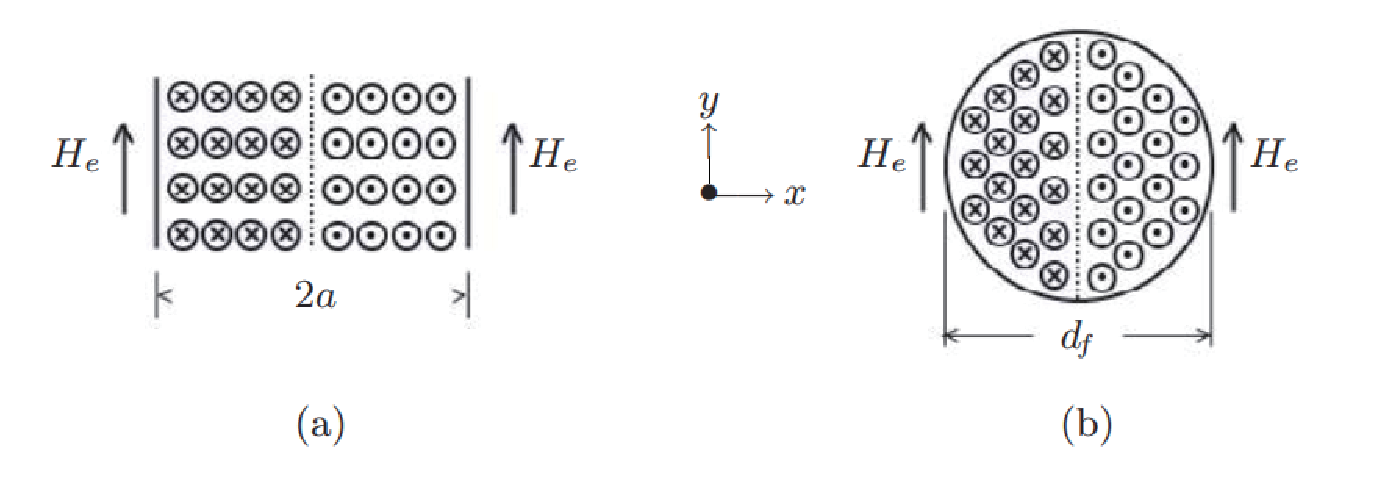
\includegraphics[scale=0.5]{chpt5/figs/fig5.16.eps}
	\caption{感应电流分布:a) 宽度为$2a$的Bean板;b)直径为$d_f$的无限长细丝。两者均置于$y$向的外场$H_e$中。}
\end{figure}

\subsection{讨论5.4:磁化中的$J_c$}
我们在此说明如何从​​磁化$M$数据中提取临界电流密度$J_c$数据。
当处理对于标准电压与电流测量技术而言太短的超导体样本时,
这种从$M$数据中提取$J_c$数据的方法非常有用。
在HTS发展的早期,测试样品因太小而不能进行$V(I)$测量,
上面讨论的Bean模型非常有用。

在$V(I)$测量中,样品必须够“长”以便:
1) 产生极小但可检测的电场,该电场定义了超导-正常转变,典型值为0.1到1 $\mu$V/ cm之间;
2) 保持测试样品两端的引线接触电阻足够“低”以防止可能导致过早正常转变的端部过热。
试样通常应至少长10 mm;某些情况下可以短到不能更短的5 mm。
最短长度在很大程度上取决于临界电流水平。

图5.8给出了10 K,20 K和30 K下的铜/$\mathrm{MgB_2}$复合线短样
(15 mm长,$\mathrm{MgB_2}$本身直径为0.531 mm,当量直径1.038 mm)[5.7]的磁化强度 vs. 外施磁场曲线。
这里,磁化单位以emu/$\mathrm{cm^3}$给出,对应直径为1.038 mm。
外场沿导线轴向,与讨论5.3第1部分中条件相同。
比如,为了计算超导体在零场、10 K下的的$J_c$,
我们将导线视为0.531 mm的无限长Bean杆。
首先,我们通过乘以系数1000将emu/$\mathrm{cm^3}$转换为SI单位(附录I)。

由图5.8可知,在零场和10K时,磁化强度为60 emu/$\mathrm{cm^3}$60 kA/m。
为了将其转换为仅对应于$\mathrm{MgB_2}$的体积的$M$,
我们必须将60 kA/m乘以$(1.038/0.531)^2 = 4.0$。
在$M$=240 kA/m,$d_f = 5.31\times10^{-4}$ m下解方程5.26,有:
\begin{align*}%page331 第5个
J_{c}(0\ \mathrm{T};10\ \mathrm{K})&=\frac{6\ \mathrm{M}(0\ \mathrm{T};10\ \mathrm{K})}{d_{f}}\\
&=\frac{6(240\times10^{3}\ \mathrm{A/m})}{(0.531\times10^{-3}\ \mathrm{m})}\\
&=2.7\times10^{9}\ \mathrm{A/m^{2}}
\end{align*}


\subsection{问题5.1:磁化测量}
该问题将5.4中讨论的磁化测量技术应用于混合III超导磁体中使用的四种超导体之一,
用以确认其不会有磁通量跳跃。
无磁通量跳跃是非低温稳定磁体的必要条件之一--- 这一点将在第6章中详细讨论。

表5.1列出了超导体的规格,这是一种裸NbTi复合带,尺寸为9.2 mm宽,2.6 mm厚。
(表格中的所有参数并非都与此问题相关,如扭绞节距等。)

测试样品是由52(13$\times$4)个100 mm长的条带组成的38 mm$\times$38 mm 方形横截面的实心矩形,如图5.17所示。
各裸带用薄带电绝缘。
在图5.17a所示的方向上,各条带的窄面置于外磁场$B_e$中;
在图5.17b所示的方向上,各条带的宽面置于外场$B_e$中。
将测试样品组合体放置在包含一个初级探测线圈和两个次级探测的矩形孔(横截面107 mm$\times$42 mm)探测线圈组内(图5.17c)。
测试组合体中平面与主探测线圈的中平面重合,
探测线圈中平面与产生$B_e$的外部磁体的中平面重合。
初级线圈和其中一个次级线圈之间的中平面到中平面距离为70 mm。
初级线圈在其中平面轴向对称绕40 mm距离内绕500匝细铜线;
各次级探测线圈有280匝,以其中平面的中心轴向延伸20 mm。
各探测线圈中轴向的匝数密度均匀。

如图5.17a取向的4.2 K测试样品,在外部磁感应$B_e$以0.05T/s的速率在0和5 T之间扫描时,
可以获得类似于图8.5的$-M$(以$V_{mz}$给出) vs. $B_e$图。
$+V_{mz}$是积分器输出,与样品磁化的负数$-M$成正比。
有效积分时间$\tau_{it}$为1 s;
平衡电位器的常数$k$为0.5。
假设电压漂移可忽略不计。

\colorbox{red}{表5.1}


\begin{figure}[htbp]
	\centering
	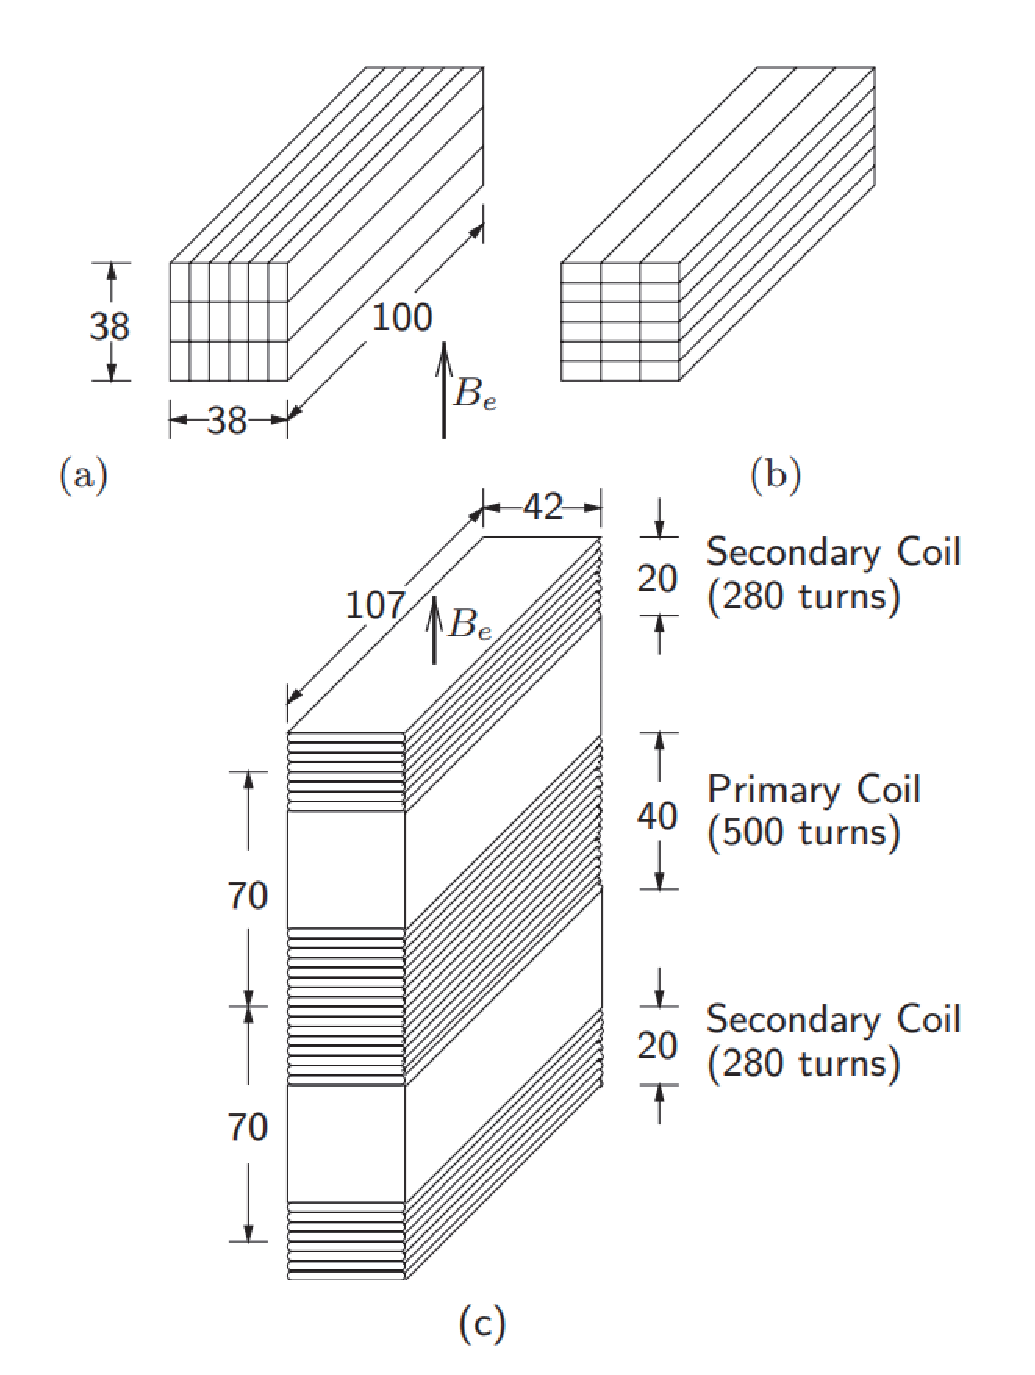
\includegraphics[scale=0.5]{chpt5/figs/fig5.17.eps}
	\caption{磁化测量细节,以mm为单位。
		(a)各带的窄面置于外场$B_e$;(b) 各带宽面置于外场$B_e$; (c) 探测线圈设置。}
\end{figure}

a) 估计$B_e\sim$2.5 T(图5.8所示的磁化轨迹宽度)下的$\Delta V_{mz}$。
注意到,$\tau_{it}$=1 s,$k$=0.5。
假设$d_f=2a$,其中$d_f$是细丝直径,$2a$是Bean板宽度。

b) 通过将低温容器中液氦压力降低到12.6 torr,进行1.8 K测量。
控制低温容器压力的技术人员发现,
当样品取向如图5.17b时,相比于图5.17a的取向,由于液氦蒸发率增加,压力控制更加越困难。
他的观察确实是否合理?试解释。

c) 探测线圈检测到的外场$B_e$的$z$分量在整个径向空间可近似表示为:
\begin{equation}%page333 第1个
B_{e}(z)\simeq B_{e}(0)[1-c(\frac{z}{z_{o}})^{2}]\qquad(5.30)
\end{equation}
其中,$z_o$ = 75 mm。
基于你有的信息,计算$c$值。 

\subsubsection{问题5.1之解}
a) 方程5.13表明探测线圈需要平衡;否则,正比于外施磁场的那一项会对视在磁化作贡献。
既然图5.8中给出的$−M(H)$迹线并非上翘,可见搜索线圈已经获得平衡。

由方程5.14b有:
\begin{align*}%page334 第1个
V_{bg}(t)=(k-1)\mu_{o}N_{pc}A_{pc}\frac{dM}{dt}\tag{5.14b}
\end{align*}

由方程5.16c,我们有:
\begin{align*}%page334 第2个
\Delta V_{mz}=-f_{m}\frac{(k-1)\mu_{o}N_{pc}A_{pc}}{\tau_{it}}J_{c}a\tag{5.16c}
\end{align*}

我们有:$k$ = 0.5; $\tau_{it}$ = 1 s; $N_{pc}$ = 500; $A_{pc}$ = (13)(0.1 m)(2.6$\times 10^{−3}$ m) = 3.38$\times 10^{−3}\ \mathrm{m^2}$ 
[(0.1 m)$\times$(38$\times 10^{−3}$ m) = 3.8$\times 10^{−3}\ \mathrm{m^2}$也是可以接受的]; $f_m$ =(NbTi体积)/(总体积)= $1/(\gamma_{c/s} + 1)$ = 0.25。

\textbf{$J_c$的估算(4.2 K,2.5 T)}

从表5.1可知,在4.2 K和5 T时的$J_c$为$2.0\times 10^9\ \mathrm{A/m^2}$。
在给定温度下,基于方程1.3获得$J_c(B_e)$的近似值是业界普遍接受的:
\begin{align*}%page334 第3个
2.0\times10^{9}\ \mathrm{A/m^{2}}=\frac{J_{0}B_{0}}{5T+0.3T}\Rightarrow J_{0}B_{0}=10.6\times 10^{9}\ \mathrm{AT/m^{2}} \tag{S1.1}
\end{align*}
式中,对NbTi,$B_0\sim$ 0.3 T。$J_0$是零场下的临界电流密度——通常是很难测量的。
于是,由5 T的$J_c$和$B_0$ = 0.3 T,我们首先可以得到$J_0 B_0$:
\begin{align*}%page334 第4个
2.0\times 10^{9}\ \mathrm{A/m^{2}}=\frac{J_{0}B_{0}}{5T+0.3T}\Rightarrow J_{0}B_{0}=10.6\times 10^{9}\ \mathrm{A/m^{2}}
\end{align*}

一旦获得了$J_0 B_0$,可以解出2.5 T时的$J_c$:
\begin{align*}%page334 第5个
J_{c}(2.5T)=\frac{10.6\times10^{9}\ \mathrm{AT/m^{2}}}{2.8T}=3.8\times 10^{9}\ \mathrm{A/m^{2}}
\end{align*}

向方程5.16c代入合适的值,有:
\begin{align*}%page334 第6个
\Delta V_{mz}&=-0.25\frac{(-0.5)(4\pi\times 10^{-7}\ \mathrm{H/m})(500)(3.38\times 10^{-3}\ \mathrm{m^{2}})}{1\ \mathrm{s}}\\
&\times(3.8\times 10^{9} A/m^{2})(50\times 1^{-6} m)\\
&\simeq 50\ \mathrm{mV}
\end{align*}

因为条带是使用圆导体经过挤压过程得到的,细丝直径在平行于$B_e$的方向实际上略小于等价
圆截面半径,即上文用于计算$\Delta V_{mz}$的a = 50 $\mathrm{\mu m}$。
 如果使用小50 $\mathrm{\mu m}$的半径, $\Delta V_{mz}$将小于50 mV。

b) NbTi细丝的各向异性的形状导致图5.17b取向下的磁化大于图5.17a取向下的磁化
---因“有效”$a$更大。
于是,会有更多大的磁化损耗。

如果细丝的纵横比和导体一样,图5.17b中的涡流损耗将正比于$(a\.{H}_e)^2$,
图5.17b中的会正比于$(b\.{H}_e)^2$---回顾问题2.8。
于是,图5.17b的涡流损耗要比图5.17a情况大$(9.2/2.6)2 = 12.5$倍。

因更高磁化损耗和涡流损耗为液氦带来的热负荷将导致更高的液氦蒸发率;
所以,技术员的观察是有道理的。

c) 探测线圈平衡时,有:
\begin{align*}%page335 第1个
N_{pc}A_{pc}(\frac{d\tilde{B}_{e}}{dt})_{pc}=N_{sc}A_{sc}(\frac{d\tilde{B}_{e}}{dt})_{sc}\tag{S1.2}
\end{align*}

因为$A_{pc} = A_{sc}$,我们有$N_{pc}[\tilde{B}_e]_{pc}=N_{sc}[\tilde{B}_e]_{sc}$。
根据对称性,我们仅考虑上半部分(下面的问题中省去了单位mm):
\begin{align*}%page335 第2个
[\tilde{B}_{e}]_{pc}=\frac{B_{e}(0)}{20}\int_{0}^{20}[1-c(\frac{z}{z_{0}})^{2}]dz\tag{S1.3a}
\end{align*}
\begin{align*}%page335 第3个
[\tilde{B}_{e}]_{sc}=\frac{B_{e}(0)}{20}\int_{60}^{80}[1-c(\frac{z}{z_{0}})^{2}]dz\tag{S1.3b}
\end{align*}

$N_{pc}[\tilde{B}_e]_{pc}=N_{sc}[\tilde{B}_e]_{sc}$等式给出:
\begin{align*}%page335 第4个
\frac{250}{20}\int_{0}^{20}[1-c(\frac{z}{z_{0}})^{2}]dz&=\frac{280}{20}\int_{60}^{80}[1-c(\frac{z}{z_{0}^{2}})]dz\\\tag{S1.4}
250[20-\frac{c}{3}\frac{(20)^{3}}{(75)^{2}}]dz&=280[80-\frac{c}{3}\frac{(80)^{3}}{(75)^{2}}-60+\frac{c}{3}\frac{(60)^{3}}{(75)^{2}}]\\
5000-118.5c&=22400-8495.4c-16800+1584c\\
c&\simeq\frac{600}{4793}\simeq 0.125
\end{align*}


\subsection{讨论5.5:磁扩散和热扩散}
在进入问题5.2研究磁通跳跃判据之前,我们先推导定义磁扩散和热扩散的基本方程:
磁扩散系数$D_{mg}$,热扩散系数$D_{th}$。
两种扩散的相对大小在正常金属中($D_{th}\gg D_{mg}$)和第II类超导体中($D_{th}\ll D_{mg}$)很不同。
第II类超导体中的$D_{th}\gg D_{mg}$使得磁通进入超导体为绝热过程,引起了磁通跳跃的判据,这将在问题5.2中研究。

为了推导磁扩散方程,要用到微分形式的Maxwell方程的安培定律和法拉第定律:
\begin{align*}%page336 第1个
\mbox{安培定律}:\quad \nabla\times\vec{H}=\vec{J}_{f}\tag{2.5}
\end{align*}
\begin{align*}%page336 第2个
\mbox{法拉第定律}:\quad\nabla\times\vec{E}=-\frac{\partial\vec{B}}{\partial t}\tag{2.8}
\end{align*}

对板状(宽度$2a$)几何,上面的方程改写为:
\begin{equation}%page336 第3个
\mbox{安培定律}: \frac{\partial H_{y}}{\partial x}=J_{z}=\frac{E_{z}}{\rho_{e}}
\end{equation}
\begin{equation}%page336 第4个
\mbox{法拉第定律}:\frac{\partial E_{z}}{\partial x}=\frac{\partial B_{y}}{\partial t}=\mu_{o}\frac{\partial H_{y}}{\partial t}
\end{equation}
其中,$\rho_e$是材料的电阻率。根据方程5.31和5.32,我们有:i
\begin{align}%page336 第5个
\rho_{e}\frac{\partial^{2}H_{y}}{\partial x^{2}}&=\mu_{o}\frac{\partial H_{y}}{\partial t}\\\notag
\frac{\rho_{e}}{\mu_{o}}\frac{\partial^{2}H_{y}}{\partial x^{2}}&\equiv D_{mg}\frac{\partial^{2}H_{y}}{\partial x^{2}}=\frac{\partial H_{y}}{\partial t}
\end{align}

方程5.33即磁扩散方程,其中:
\begin{equation}%page336 第7个
D_{mg}=\frac{{\rho}_{e}}{\mu_{o}}
\end{equation}

类似的,热物性为常数的一维热扩散方程为:
\begin{equation}%page336 第8个
k\frac{\partial^{2}T}{\partial x^{2}}=C\frac{\partial T}{\partial t}
\end{equation}
其中,$k$和$C$分别是材料的热导率和热容。
方程5.35两侧分别除以$C$,有:
\begin{align*}%page336 第9个
\frac{k}{C}\frac{\partial^{2}T}{\partial x^{2}}\equiv D_{th}\frac{\partial^{2}T}{\partial x^{2}}=\frac{\partial T}{\partial t}\tag{5.35b}
\end{align*}

方程5.35b即热扩散方程,其中:
\begin{equation}%page336 第10个
D_{th}=\frac{k}{C}\qquad(5.36)
\end{equation}

我们注意到方程5.36和4.20是等价的,因为$C=\rho c_p$。

\colorbox{red}{表5.2}


表5.2列出了不锈钢和铜在​​4 K和80 K时的电气和热物性以及相应的扩散系数的近似值。
从表5.2中我们可以清楚地看到,
不锈钢(用于近似正常态超导体)和铜在磁性和热扩散性方面是相反的。
具体而言,磁场的变化在不锈钢中传播快,而温度梯度的传播相对较慢;
因此,在磁场变化期间,锈钢中将产生很大的不均匀温度分布。
物理上看,这意味着在第II类超导体中的磁加热基本是绝热进行的。
在铜中,情况正好相反:磁场扩散非常缓慢,而温度的任何不均匀性都很快“被均化”。
因此,与第II类超导体紧密接触的铜可以减轻第II类超导体因磁场变化引起的不稳定性。
这种考虑是动态稳定性的本质,是1960和1970年代发展起来的稳定性标准之一[5.8],
也适用于1980年代后期的HTS [5.9]。

\subsection{问题5.2:磁通跳跃判据}
本问题推导产生磁通跳跃的导体的临界导尺寸。
1960年代早期,磁通跳跃曾经是第一个具有工程意义的超导磁体的不稳定性的主要来源[5.10]。
 磁通跳跃是允许磁场穿透其内部的第II类超导体特有的热不稳定性,
 导体表面上的时变磁场$\.{H}_e$在导体内感应出电场$\vec{E}$,
 电场与超导电流(密度$J_c$)相互作用($\vec{E}\cdot \vec{J}_c$)会加热超导体。
由于$J_c$随温度升高而降低,磁场(磁通量)进一步进入到超导体中,产生更多热量,这又进一步降低$J_c$。
 场穿透和温升可以交叠,直到超导体失去其超导电性。 这种热失控事件称为磁通跳跃。


a) 使用Bean模型,计算板正半部分($0\le x\le a$)的$\vec{E}\cdot \vec{J}_c$,
证明在临界电流密度$J_c$突然减掉$|\Delta J_c|$时,,板内部耗散能量密度$e_\phi$[J/m3]为:
\begin{equation}%page338 第1个
e_{\phi}=\frac{\mu_{o}J_{c}|\Delta J_{c}|a^{2}}{3}
\end{equation}

我们注意到,处于临界态的整个板的表面($\pm a$)暴露于外场$H_e\vec{i}_y$中。

b) 通过计算流入板$x=a$处的Poynting能流,并令之与板的正半部分的储存和耗散能量$\mathcal{E}_\phi$相等
推导出5.37。 

c) 为了将$\Delta J_c$与导体的等效温升联系起来,我们可以假设$J_c(T)$与温度为线性关系:
\begin{equation}%page338 第2个
J_{c}(T)=J_{c_{o}}(\frac{T_{c}-T}{T_{c}-T_{op}})
\end{equation}
其中,$J_{c_o}$是运行温度$T_{op}$下的临界电流密度。
$T_c$是给定磁场$B_{o}$下的临界温度。
由5.38,方程5.37中的$\Delta J_c$可以与等效温升$\Delta T$联系起来:
\begin{equation}%page338 第3个
\Delta J_{c}=-J_{c_{o}}(\frac{\Delta T}{T_{c}-T_{op}}
\end{equation}
现在,通过要求 $\Delta T_s=e_\phi/\~{C}_s\le \Delta T$,说明
热稳定性要求板的临界宽度$a_c$为下式。其中,$\~{C}_s$是超导体在温度$T_{op}$和$T_c$之间
的平均热容:
\begin{equation}%page338 第4个
a_{c}=\sqrt{\frac{3\tilde{C}_{s}(T_{c}-T_{op})}{\mu_{o}J_{c_{o}}^{2}}}
\end{equation}


\subsubsection{问题5.2之解}
a) 因为关于$x=0$对称,我们仅考虑板在$x=0$和$x=a$之间的部分。
如图5.18所示,实线对应$H_{s1}(x)$,它给出了在$J=J_c$下板内的初始场分布。
点线对应板载流为$J_c-|\Delta J_c|$时的$H_{s2}(x)$。
注意到两种情况下,在表面上磁场均为$H_e$。于是我们有:
\begin{align*}%page339 第1个
H_{s1}(x)=H_{e}+J_{c}(x-a)\tag{S2.1a}
\end{align*}
\begin{align*}%page339 第2个
H_{s2}(x)=H_{e}+(J_{c}-| \Delta J_{c}|)(x-a)\tag{S2.1b}
\end{align*}
\begin{figure}[htbp]
	\centering
	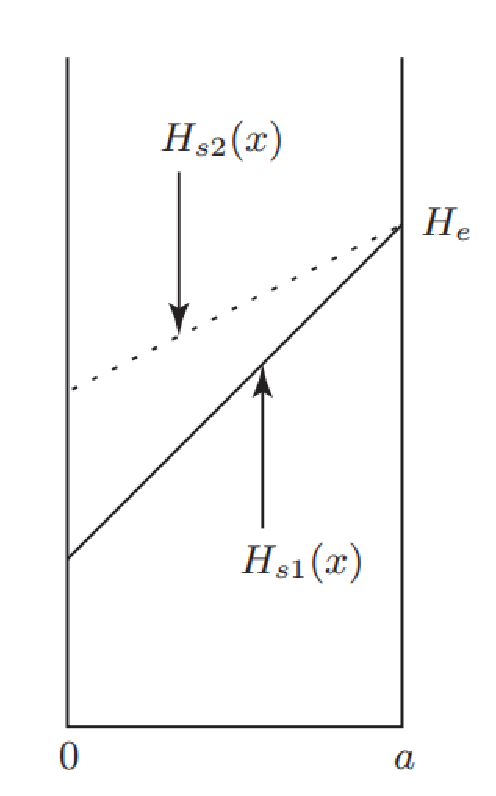
\includegraphics[scale=0.5]{chpt5/figs/fig5.18.eps}
	\caption{磁场特征。}
\end{figure}

因为板内有磁场的变化,将产生电场$\vec{E}$。根据Faraday感应定律,有:
\begin{align*}%page339 第3个
\oint_{C}\vec{E}\cdot d\vec{s}=-\mu_{o}\int_{S}\frac{\triangle H_{s}(x)\vec{\imath}_{y}\cdot d\vec{A}}{\Delta t} \tag{S2.2}
\end{align*}

根据对称性,我们有$\vec{E}(x = 0) = 0$,$\vec{E}$指向$z$向。
$\Delta H_s(x)$由下式给出:
\begin{align*}%page339 第4个
\Delta H_{s}(x)&=H_{s2}(x)-H_{s1}(x)\\
&=|\Delta J_{c}|(a-x)\tag{S2.3}
\end{align*}

联立方程S2.2和S2.3,有:
\begin{align*}%page339 第5个
E_{z}(x)&=\mu_{o}\frac{|\Delta J_{c}|}{\Delta t}\int_{0}^{x}(a-x)dx\\
&=\mu_{o}\frac{|\Delta J_{c}|}{\Delta t}(ax-\frac{x^{2}}{2})\tag{S2.4}
\end{align*}

耗散能量密度$p(x)$为$E_z(x)J_c$;
板内耗散的单位长度能量密度或$y-z$平面上的单位表面积能量密度$\mathcal{E}_\phi[\mathrm{J/m^2}]$]为:
\begin{align*}%page339 第6个
\varepsilon_{\phi}&=\int_{0}^{a}p(x)\Delta tdx\\
&=\mu_{o}J_{c}|\Delta J_{c}|\int_{0}^{a}(ax-\frac{x^{2}}{2})dx=\frac{\mu_{o}J_{c}|\Delta J_{c}|a^{3}}{3}\tag{S2.5}
\end{align*}

平均耗散能量密度$e_\phi$由$\mathcal{E}_\phi/a$ 给出:
\begin{align*}%page339 第7个
e_{\phi}=\frac{\mu_{o}J_{c}|\Delta J_{c}|a^{2}}{3}\tag{5.37}
\end{align*}

b) $y-z$平面上在$x=a$处进入板($+x$方向)的Poynting能流
等于板内储存的磁能$\delta E_m$的变化量和板内耗散的能流$\mathcal{E}_\phi$: 
\begin{align*}%page340 第1个
\int S_{x}(a)dt=\Delta E_{m}+\varepsilon_{\phi}\tag{S2.6}
\end{align*}

通过在$x=a$处计算$\vec{S}=\vec{E}\times\vec{H}$可以确定$\vec{S}$的方向。在$x=a$处,
$\vec{H}=H_e \vec{i_y}$;由方程S2.4得到的$E_z(x)$,可得:
\begin{align*}%page340 第2个
E_{z}(a)=\mu_{o}\frac{|\Delta J_{c}|a^{2}}{2\Delta t}\tag{S2.7}
\end{align*}

于是:
\begin{align*}%page340 第3个
\vec{S}(a)=\mu_{o}\frac{|\Delta J_{c}|a^{2}}{2\Delta t}\vec{\imath}_{z}\times H_{e}\vec{\imath}_{y}=-\mu_{o}\frac{H_{e}|\Delta J_{c}|a^{2}}{2\Delta t}\tag{S2.8}
\end{align*}

如我们所料,$\vec{S}(a)$指向$−x$向;能流流入板内。于是:
\begin{align*}%page340 第4个
\int S_{x}(a)dt=\mu_{o}\frac{H_{e}|\Delta J_{c}|a^{2}}{2}\tag{S2.9}
\end{align*}

板内磁能通量的差值$\Delta E_m$为:
\begin{align*}%page340 第5个
\Delta E_{m}&=\frac{\mu_{o}}{2}\int_{0}^{a}[H_{s2}^{a}(x)-H_{s1}^{2}(x)]dx\\\tag(S2.10)
&=\frac{\mu_{o}}{2}\int_{0}^{a}\{[H_{e}+(J_{c}-|\Delta J_{c}|)(x-a)]^{2}-[H_{e}+J_{c}(x-a)]^{2}\}dx\\
&=\frac{\mu_{o}}{2}\int_{0}^{a}[-2H_{e}|\Delta J_{c}|(x-a)-2J_{C}|\Delta J_{c}|(x-a)^{2}+|\Delta J_{c}|^{2}(x-a)^{2}]dx
\end{align*}

忽略上面的积分中的$|\Delta J_c|^2$项,有:
\begin{align*}%page340 第6个
\Delta E_{m}=\mu_{o}(\frac{H_{e}|\Delta J_{c}|a^{2}}{2}-\frac{J_{c}|\Delta J_{c}|a^{3}}{3})\tag{S2.11}
\end{align*}

从S2.6,我们有:
\begin{align*}%page340 第7个
\varepsilon_{\phi}=\int S_{x}(a)dt-\Delta E_{m}\tag{S2.12}
\end{align*}

联立S2.9,S2.11和S2.12,我们得到:
\begin{align*}%page340 第8个
\varepsilon_{\phi}&=\mu_{o}\frac{H_{e}|\Delta J_{c}|a^{2}}{2}-\mu_{o}(\frac{H_{e}|\Delta J_{c}|a^{2}}{2}-\frac{J_{c}|\Delta J_{c}|a^{3}}{3})\\
&=\mu_{O}\frac{J_{c}|\Delta J_{c}|a^{3}}{3}\tag{S2.13}
\end{align*}
方程S2.13直接可以导出5.37:
\begin{align*}%page340 第9个
e_{\phi}=\frac{\varepsilon_{\phi}}{a}=\frac{\mu_{o}J_{c}|\Delta J_{c}|a^{2}}{3}\tag{5.37}
\end{align*}

c)  5.38已给出,$J_c(T)$是随温度增加而减小的。于是,我们有
\begin{align*}%page341 第1个
\Delta J_{c}=-J_{c_{c}}(\frac{\Delta T}{T_{c}-T_{op}})\tag{5.39}
\end{align*}

由5.39,得:
\begin{align*}%page341 第2个
|\Delta J_{c}|=\frac{J_{c_{o}}\Delta T}{T_{c}-T_{op}}\tag{S2.14}
\end{align*}

在方程5.37中,使用$J_{c_o}$代替$J_c$。与S2.14联立,得到:
\begin{align*}%page341 第3个
e_{\phi}=\frac{\mu_{o}J_{c_{o}}^{2}\Delta T a^{2}}{3(T_{c}-T_{op})}\tag{S2.15}
\end{align*}

注意到,$e_{\phi}$不仅正比于$\Delta T$,而且正比于$a^2$(更重要)。
在绝热条件下,耗散能量密度$e_{\phi}$引起超导体温度升高$\Delta T_s$:
\begin{align*}%page341 第4个
\Delta T_{s}=\frac{e_{\phi}}{\tilde{C}_{s}}>0\tag{S2.16}
\end{align*}
其中,$\tilde{C}_{s}$是超导体在温度$T_{op}$到$T_c$之间的平均热容。
联立S2.15和S2.16,热稳定要求$\Delta T_s <\Delta T$,于是有:
\begin{align*}%page341 第5个
\frac{\Delta T_{s}}{\Delta T}<\frac{\mu_{o}J_{c_{o}}^{2}a^{2}}{3\tilde{C}_{s}(T_{c}-T_{op})}\tag{S2.17}
\end{align*}

对一个给定的超导材料和运行温度,$a$是用以满足S2.17的唯一可变的磁体设计参数。
也即,热稳定性仅在板的半宽度$a$小于临界尺寸$a_c$时才能满足:
\begin{align*}%page341 第6个
a_{C}=\sqrt{\frac{3\tilde{C}_{s}(T_{c}-T_{op})}{\mu_{o}J_{c_{o}}^{2}}}\tag{5.40}
\end{align*}

将方程5.40应用于计算运行于4.2 K的NbTi和运行于77.3 K的YBCO的近似$a_c$值。
 表5.3列出了上述两种超导体与方程5.40有关的近似参数。

我们可以得到如下结论:NbTi圆形细丝,$a_c=140\ \mathrm{\mu m}$意味着临界直径为
$\sim 300\ \mathrm{\mu m}$;对图层YBCO带材,临界宽度为8 mm。

\colorbox{red}{表5.3}

\subsection{问题5.3:磁通跳跃}
图5.19所示的磁化 vs. 外场曲线是Nb-Zr单丝($\phi=$0.5 mm)在4.2 K无传输电流
的条件下获得的。 (1960年代早期,Nb-Zr合金超导体要比Nb-Ti更早。
在1960年代中期复合超导体成为磁体级超导体的标准形式后,
Nb-Ti(现在更习惯写成NbTi),NbTi因其和铜更容易一起处理,取代了Nb-Zr。
注意到,纵坐标(磁化)和横坐标(磁场)都是以非SI单位给出的。
使用Bean模型,将直径为$d_f$的金属丝视为厚度为$2a$的板。

a) 证明曲线中的磁场区间$\Delta H_f$与测到的磁化强度幅值一致。

b) 估算图5.19中标A处磁通跳跃因其的耗散能量密度$e_{\phi}\ [\mathrm{J/m^3}]$。
首先,证明$e_{\phi}$可由下式给出:
\begin{equation}%page342 第1个
e_{\phi}=\frac{(\mu_{o}J_{p})^{2}}{6\mu_{o}}
\end{equation}

c) 估计磁通跳跃A因其的温升。
假设Nb-Zr热容与温度无关,为6 $\mathrm{kJ/m^3 K}$。

\begin{figure}[htbp]
	\centering
	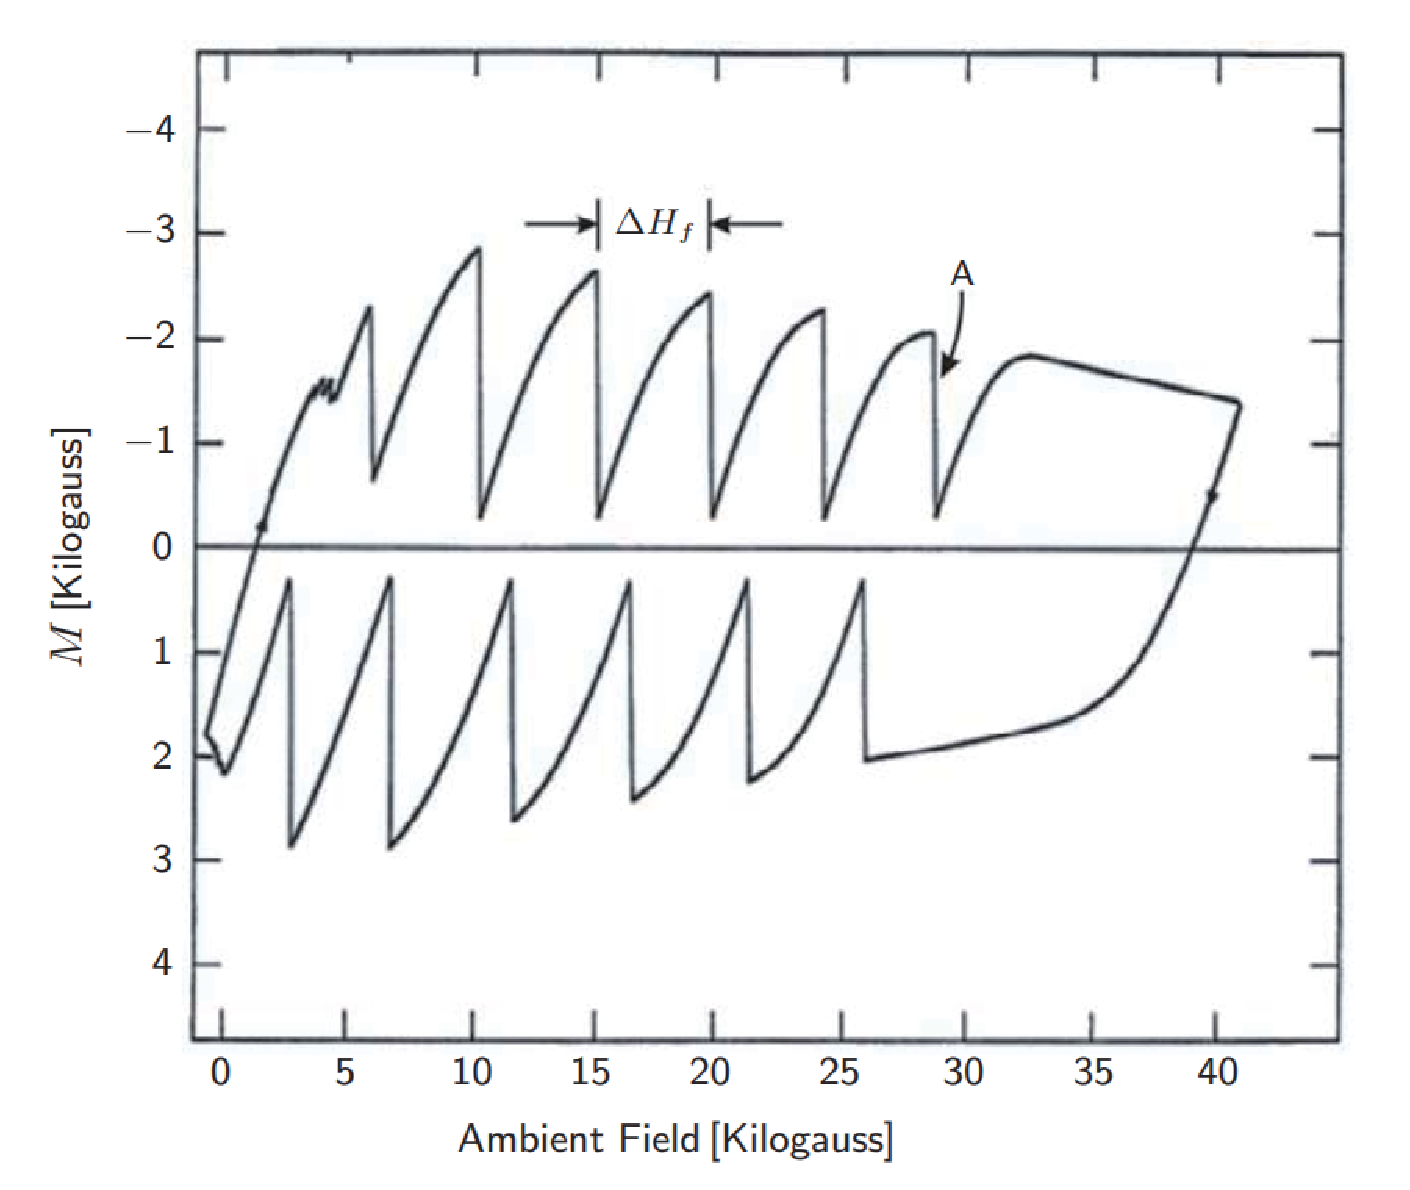
\includegraphics[scale=0.5]{chpt5/figs/fig5.19.eps}
	\caption{0.5 mm直径Nb-Zr单丝的磁化 vs. 外场曲线。}
\end{figure}


\subsubsection{问题5.3之解}
a) 根据Bean模型,磁通跳跃可在任意$H_p$下发生。
显然,有$H_p = \Delta H_f$,其中,$\Delta H_f$如图5.19所示。
同时,板的完全磁化为$H_p/2$。

从图5.19可知,$\Delta H_f\simeq$ 5 k gauss,$\mu_{0}\Delta H_f$=0.5 T。图中还给出,
$H_p/2\simeq$ 2.5 k gauss,是$\Delta H_f$的一半。他们是一致的。

b) 我们可以使用Poynting能量平衡$e_s=e_{\phi}+\Delta e_m$推导出磁通跳跃能量密度$e_{\phi}$,
其中,$e_s$是在$x=a$处进入超导体的Poynting能量密度, $\Delta e_m$是储存的能量密度的变化量。
我们仅考虑$0\le x\le a$部分。板内的$\Delta H(x)$为:
\begin{align*}%page343 第1个
\Delta H(x)=H_{p}\frac{(a-x)}{a}\tag{S3.1}
\end{align*}

由S3.1,可得:
\begin{align*}%page343 第2个
E(x)=\mu_{o}\frac{H_{p}}{\Delta t}\int_{0}^{x}\frac{a-x}{a}dx=\frac{\mu_{o}H_{p}}{a\Delta t}(ax-\frac{x^{2}}{2})\tag{S3.2}
\end{align*}

这样,在$x=a$处$\vec{S}$为:
\begin{align*}%page343 第3个
\vec{S}(a)=-\frac{\mu_{o}}{2\Delta t}H_{p}aH_{e}\vec{\imath}_{x}\tag{S3.3}
\end{align*}

$\vec{S}(a)$朝向板,Poynting能量密度由下式给出:
\begin{align*}%page343 第4个
e_{s}=\frac{\int S_{x}(a)dt}{a}=\frac{\mu_{o}}{2}H_{p}H_{e}\qquad(S3.4)
\end{align*}

磁通跳跃($e_{m2}$)后储存的磁能密度为$\mu_o H_e^2/2$。
磁通跳跃前储存的磁能密度$e_{m1}$为: 
\begin{align*}%page343 第5个
e_{m1}=\frac{\mu_{o}}{2a}\int_{0}^{a}[H_{e}+J_{c}(x-a)]^{2}dx\tag{S3.5}
\end{align*}
积分展开,
\begin{align*}%page343 第6个
e_{m1}=\frac{\mu_{o}}{2a}(H_{e}^{2}a-H_{e}J_{c}a^{2}+\frac{J_{c}^{2}a^{3}}{3})=\frac{\mu_{o}}{2}H_{e}^{2}-\frac{\mu_{o}}{2}H_{e}H_{p}+\frac{\mu_{o}}{6}H_{p}^{2}\tag{S3.6}
\end{align*}
\begin{align*}%page343 第7个
\Delta e_{m}=e_{m2}-e_{m1}=\frac{\mu_{o}}{2}H_{e}H_{p}-\frac{\mu_{o}}{6}H_{p}^{2}\tag{S3.7}
\end{align*}

因为$e_\phi=e_s-\Delta e_m$,我们有:
\begin{align*}%page343 第8个
e_{\phi}=\frac{\mu_{o}}{2}H_{p}H_{e}-\frac{\mu_{o}}{2}H_{e}H_{p}+\frac{\mu_{o}}{6}H_{p}^{2}=\frac{\mu_{o}}{6}H_{p}^{2}\tag{S3.8}
\end{align*}

方程S3.8可以写为:
\begin{align*}%page343 第9个
e_{\phi}=\frac{(\mu_{o}H_{p})^{2}}{6\mu_{o}}\tag{5.41}
\end{align*}

将$\mu_o H_p$=0.5 T代入方程5.41:
\begin{align*}%page343 第10个
e_{\phi}\simeq\frac{(0.5T)^{2}}{(6)(4\pi\times10^{-7}\ \mathrm{H/m})}\simeq33\times10^{3}\ \mathrm{J/m^{3}}
\end{align*}

c) $e_\phi = C_s \Delta T_s;33\times 10^3= 6\times 10^3 \Delta T_s$。我们解得:
$\Delta T_s$=5.5 K。这足以令超导体进入正常态了。


\subsection{问题5.4:导线换位}
如问题5.2中所讨论的,为了避免磁通跳跃,要求导体直径要小于$2a_c$,对NbTi,该值为$\sim 250\ \mathrm{\mu m}$。NbTi线的典型$J_{c_o}$是$2\times 10^9\ \mathrm{A/m^2}$(4.2 K和5 T),
$250\ \mathrm{\mu m}$直径的线的临界电流仅为$\sim 100$ A——如果使用单线,对大多数磁体应用都是不够的。
1960s末提出了使用多根线制造导体的思想:每一根线足够细以避免产生磁通跳跃,而后附着与常规金属上。
这种方法当时就造出来高达1000 A临界电流的线。现在已经可以造出50 kA的导体了。

在早期(约1969年)的“复丝”导体中,导线未加捻。
尽管每根细丝足够小以满足尺寸标准(方程5.40),但细丝之间的耦合会导致导线整体的磁通跳跃。
问题5.5涉及此类导体。
Wilson等1960年代后期在卢瑟福实验室进行的多层导体的分析和实验研究的结果开启了多丝导体的新时代[5.11]。

简单地说,当细丝嵌入导电金属(例如铜)内置于时变磁场中时,
根据Faraday定律,细丝之间是电耦合的。
然后它们作为单个实体,其有效导体直径几乎与整个导体的直径一样大。
因此,孤立细丝的磁通跳跃标准的基本前提不适用于无捻多丝导体。
为了消除多丝导体中的磁通跳跃,必须将细丝去耦。
细丝绞合,或者更理想地,将长丝(或多股导体的股线)换位可以实现细丝去耦。

考虑一个由两个宽为$d_f$的Bean板组成的二维导体模型,由宽度为$2w$、电阻率为$\rho_{cu}$的铜板
隔开。图5.20给出了从z轴向下看的导体几何。
我们注意到,与在$y$和$z$方向都无限延伸的一维Bean板不同,该导体在$y$向长$2\ell$。

\begin{figure}
	\centering
	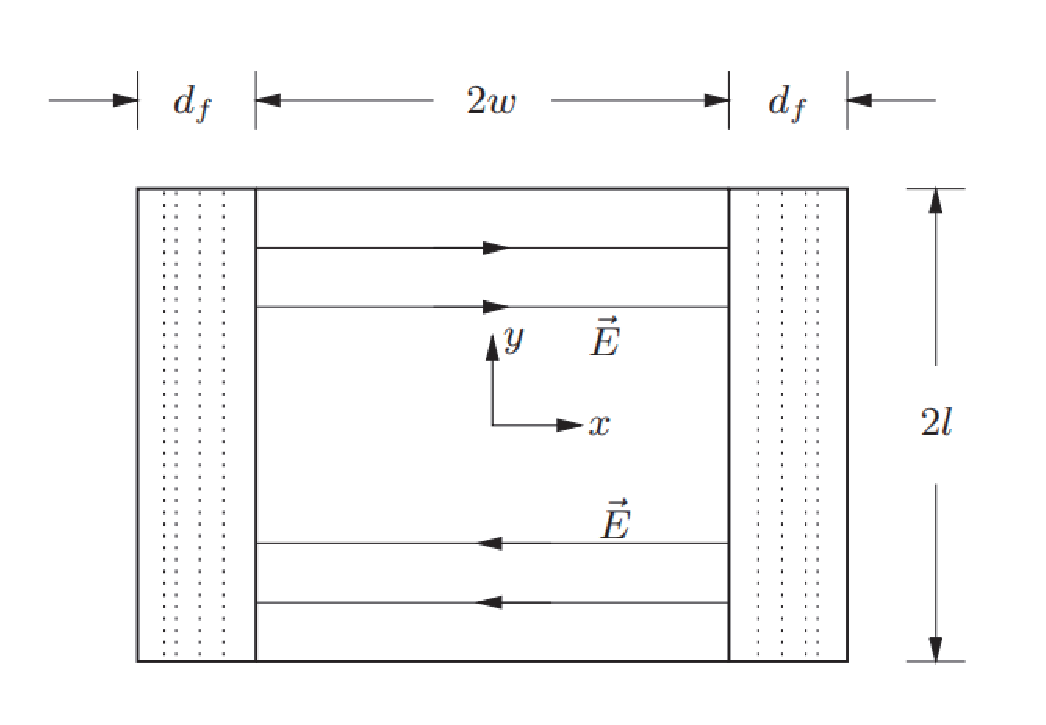
\includegraphics[scale=0.6]{chpt5/figs/fig5.20.eps}
	\caption{两个Bean板间夹正常金属板的三明治形状的二维导体。}
\end{figure}

假设导体置于指向$z$向的空间均匀时变磁场$\.{H}_{0z}\vec{i_z}$中。

a) 证明铜板内的$x$向电场$E_{1x}$按下式随$y$变化:
\begin{equation}%page345 第1个
E_{1x}=\mu_{o}\dot{H}_{0z}y\qquad(5.42)
\end{equation}
假设各超导板中的电场为零---严格说,并不是零,但与铜比,远小于铜;
因此,将电场近似为零时合理的。
同时假设场是准静态的。在这些假设下,很明显,方程5.42给出的铜中的电场仅有$x$分量。

b) 证明在一半导体长度上(从$y=0$到$y=\ell$),
从一个超导体板通过铜($z$向单位导体深度)的流向另一个超到板的净电流$I_{cp}$为:
\begin{equation}%page345 第2个
I_{cp}=\int_{0}^{\ell}J_{cu}dy=\frac{\mu_{o}\dot{H}_{0z}}{\rho_{cu}}\int_{0}^{\ell}ydy=\frac{\mu_{o}\dot{H}_{0z}\ell^{2}}{2\rho_{cu}}\quad(5.43)
\end{equation}

c) 在临界长度 $\ell_c$时,5.43给出的净电流等于板(单位导体深度)的临界电流$J_cd_f$。
证明临界长度$\ell_c$为:
\begin{equation}%page345 第3个
\ell_{c}=\sqrt{\frac{2\rho_{cu}J_{c}d_{f}}{\mu_{o}\dot{H}_{0z}}}\qquad(5.44)
\end{equation}

d) 应用于60 Hz的多丝超导体的实习尺寸$d_f$必须很小,
在$0.1\sim 0.5\ \mathrm{\mu m}$之间,这比可见光的波长($\sim 0.7\ \mathrm{\mu m}$)都小。
要求这么小的尺寸是为了各细丝在时变磁场下产生的的磁滞能量可控。
(第六章将讨论,磁场一个周期内的磁滞损耗正比于细丝直径。)

计算一个典型的微丝超导体的$\ell_c$,其参数为:
$\rho_m=$ n$\Omega$m;$J_c=2\ \mathrm{GA/m^2}$;
$d_f=0.2\ \mathrm{\mu m}$;
$\mu_o \.{H}_{0z}$=2 kT/s
(等价于60 Hz的幅值为5 T的磁场正弦激励)。
$\rho_m$是基底(通常是铜-镍合金)的电阻率。


e) 计算临界电流为100 A的0.2 $\mu$m细丝所要求的微丝数量。
和d)使用相同的参数值。

\subsubsection{问题5.4之解}
a) 根据Faraday定律,在准静态假设下,有:
\begin{align*}%page346 第1个
\frac{\partial E_{1y}}{\partial x}-\frac{\partial E_{1x}}{\partial y}=-\mu_{o}\dot{H}_{0z}\tag{S4.1}
\end{align*}

因为在超到板中$\vec{E}$为零,即在$x =\pm w$时有$E_y = 0$。这会迫使在铜板内处处$E_{1y} = 0$。
所以:
\begin{align*}%page346 第2个
E_{1x}=\mu_{o}\dot{H}_{0z}y\tag{5.42}
\end{align*}

b) 电场E已知后,铜板中的电流密度$J_{cu}$由下式给出:$J_{cu} = E_{1x}/\rho_{cu}$。
在导体长度的一半上,从一个超到板经铜板流入另一个超到板的净电流为:
\begin{align*}%page346 第3个
I_{cp}=\int_{0}^{\ell}J_{cu}dy=\frac{\mu_{o}\dot{H}_{0z}}{\rho_{cu}}\int_{0}^{\ell}ydy=\frac{\mu_{o}\dot{H}_{0z}\ell^{2}}{2\rho_{cu}}\tag{5.43}
\end{align*}

c) 令5.43给出的$I_{cp}$与$J_c d_f$相等,解出$\ell_c$,我们有:
\begin{align*}%page346 第4个
\ell_{c}=\sqrt{\frac{2\rho_{cu}J_{c}d_{f}}{\mu_{o}\dot{H}_{0z}}}\tag{5.44}
\end{align*}

d) 向5.44中代入合适的值,有:
\begin{align*}%page346 第4个
\ell_{c}=110\ \mathrm{\mu m}
\end{align*}

于是,在典型的微丝中绞合长度为$\sim$100 $\mu$m。
这意味着出于机械性要求,细丝直径应该$\sim$1 $\mu$m;
实际上,一个类似于磁通跳跃标准的热-磁稳定性标准要求它甚至要比$\sim$1 $\mu$m还细。
这是由于为了降低耦合损耗,细丝使用了Cu-Ni合金作为基底材料,导致磁扩散时间常数
小于热扩散时间常数。

e) 临界电流($I_c$),临界电流密度($J_c$),细丝数 ($N_f$ )和直径($d_f$)通过下式联系在一起:
\begin{align*}%page346 第4个
I_c=N_f\frac{\pi d_f^2}{4} J_c \tag{S4.2}
\end{align*}

向S4.2代入合适的参数,解出$N_f$:
\begin{align*}%page346 第5个
N_{f}&=\frac{4I_{c}}{\pi d_{f}^{2}J_{c}}=\frac{4(100A)}{\pi(0.2\times10^{-6}m)^{2}(2\times10^{9}A/m^{2})}\\
&=1.6\times 10^{6}
\end{align*}

为微丝导体中,微丝的数量要求接近1000万。



\subsection{问题5.5:导体磁化}
本问题示例了细丝的尺寸各绞绕对磁化的影响。
1960年代末,对同体积的三种NbTi复合导体进行了磁化测量[5.12]。
导体1,2,和3分别是:绞合的多丝线,节距长度$\ell_{p1}$;绞合的多丝线,节距长度$\ell_{p2}>\ell_{p1}$;
单丝。

图5.21给出的三种NbTi导体的磁化曲线对应,标记为A,B和C。
各导体置于图中用箭头标识的磁场脉冲中。
曲线A,B和C不一定分别对应导体1,2和3。
注意曲线B($B_1,B_2,B_3$)显示了磁场扫描速度的影响;
曲线C与磁场扫描速度无关;
曲线A也与磁场扫描速度无关,但显示了磁场脉冲引起的部分磁通跳跃。

a) 指出各曲线分别对应哪个导体。

b) 估算单丝导体与多丝导体的直径比。

c) 估算$\ell_{p2}$。导体1和2的$J_cd_f = 4\times 10^4$ A/m。
同时评价$\ell_{p1}$。

\begin{figure}
	\centering
	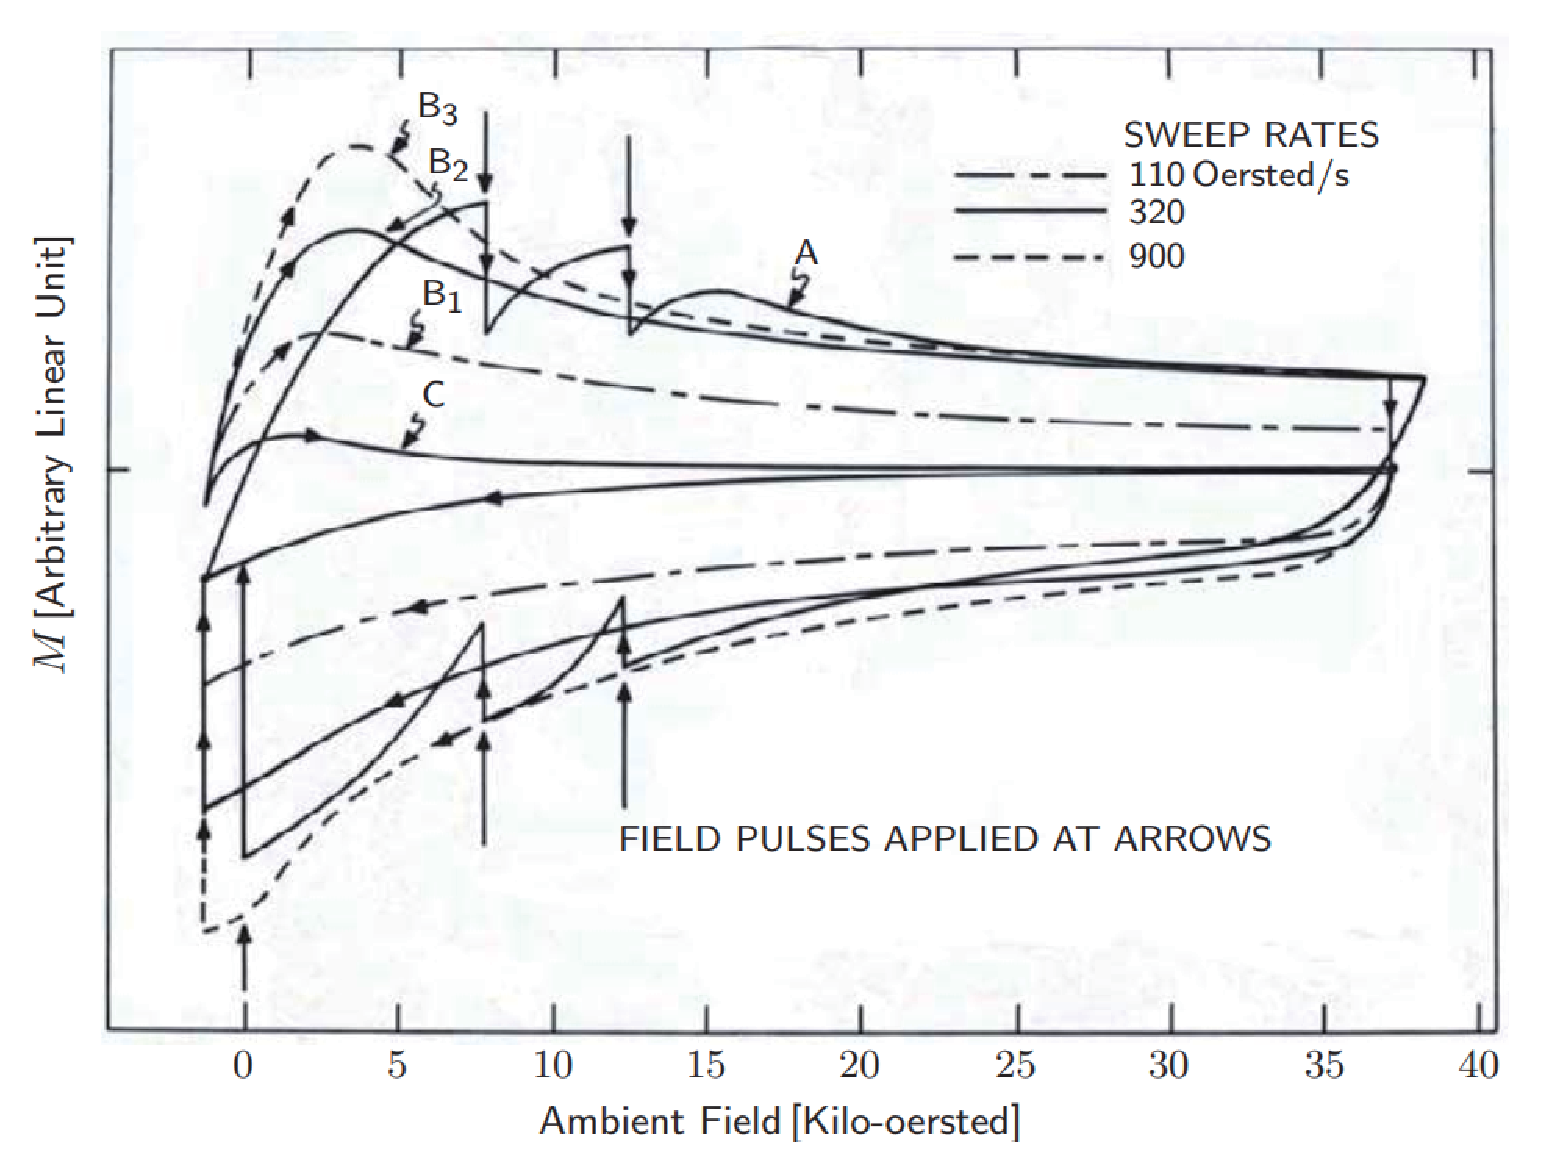
\includegraphics[scale=0.4]{chpt5/figs/fig5.21.eps}
	\caption{导体1,2,3的磁化曲线。}
\end{figure}


\subsubsection{问题5.5之解}
a) 曲线A和C与磁场扫描速率无关,对应的磁化---
可以反映出细丝直径---A比C更大。
因此,可以得出,曲线A对应导体3(单丝),曲线C对应导体1($\ell_{p1}$).。
另一个曲线B则为导体2 ($\ell_{p2}$)。 (各导体体积相同,于是,测到的磁化应该直接正比于细丝直径。)

b) 导体3的磁化宽度($M(H_e\uparrow) − M(H_e\downarrow)$,曲线A) 与导体1的(曲线C)之比
在$\mu_o H_e$小于$\sim 1$ T时,约为10.
因此,我们的结论是细丝直径比约为10。

c) 因为在900 oersted/s ($\mu_0 \.{H}_{0z}$= 0.09 T/s) 的磁场扫描速度下,导体2的曲线$B_3$
与导体3的曲线A近似相等,于是,我们得到这个磁场扫描速率对应导体2的细丝临界节距$\ell_{p2}$。
于是,由方程5.44得:
\begin{align*}%page348 第1个
\ell_{p2}=2\sqrt{\frac{2\rho_{cu}J_{c}d_{f}}{\mu_{o}\dot{H}_{0z}}} \tag{S5.1}
\end{align*}

代入$\rho_{cu}= 2\times 10^{−10}\ \mathrm{\Omega m}$;
$J_cd_f = 4\times 10^4$ A/m;
以及$\mu_o \.{H}_{0z}$= 0.09 T/s,我们得到:
\begin{align*}%page348 第2个
\ell_{p2}&=2\sqrt{\frac{(2)(2\times 10^{10}\ \mathrm{\Omega m})(4\times 10^{4}\ \mathrm{A/m})}{0.09\ \mathrm{T/S}}}\\
&=2.7\times 10^{-2}\ \mathrm{m}=27\ \mathrm{mm}
\end{align*}

这个值与实际节距值10 mm很接近。
因为导体1在扫描速率320 oersted/s下的磁化远小于导体2在同等磁场扫描速率下的值,我们
得到$\ell_{p1}$远小于$\ell_{p2}$。

\subsection{讨论5.6:换位}

推导5.44的条件$I_{cp} = J_c d_f$的一个重要内涵是两个超导板是电气耦合的。
换句话说,如果导体长度远小于$2\ell_{c}$,两导体将解耦。
实际上,哪怕各板长度远长于$2\ell_{c}$,只要他们以小于$2\ell_{c}$的节距换位,也能解耦。
在多丝导体中,我们通过以$\ell_p\ll 2\ell_{c}$的节距绞合细丝实现部分解耦;
$2\ell_{c}$在$\.{H}_{0z}$大的时候足够小。
注意到,一个绞合导体中,各细丝从保持一个与轴固定的径向距离。
反过来,在一个换位股线的电缆中,可以实现更彻底的解耦,因为当股线换位时,
各股线在电缆的螺旋时,会占据电缆直径上的每一个径向位置。


\subsection{讨论5.7:HTS中的磁通跳跃?}
\subsubsection*{A. “完全”磁通跳跃的尺度判据}

LTS的导体尺寸标准(方程5.40)最初是在$\Delta e_\phi/\Delta T=C_s$极限下得到的,
其中,$C_s$导体单位体积的热容,假定为常数。
因为LTS中,在一个完全的磁通跳跃下,温度漂移$T_c−T_{op}$很小,
这个尺寸判据足够了。

在绝热情况下抑制磁通跳跃的一般条件是超导体的磁能必须小于其热能。
在绝热情况下,除非$T_{op}$下的初始磁能密度$e_\phi(T_{op})$超过
将超导体从$T_{op}$加热到$T_c$所需的热能,否则磁通跳跃不会发展完全。
\begin{equation}%page349 5.45
e_{\phi}(T_{op})\geq h_{s}(T_{c})-h_{s}(T_{op})
\end{equation}
式中,$h_s(T_c)$和$h_s(T_{op})$分别是在$T_c$和$T_{op}$时的超导体的焓。
因为$e_\phi(T_{op})=[\mu_o H_p(T_{op})]^2/6\mu_o$ ,
对Bean板有$H_p(T_{op})=aJ_c(T_{op})$,所以,
为了抑制完全磁通跳跃,导体尺寸判据为:
\begin{equation}%page349 第2个
a_{c}=\sqrt{\frac{6[h_{s}(T_{c})-h_{s}(T_{op})]}{\mu_{o}J_{c}^{2}(T_{op})}}
\end{equation}

对比这两个尺寸判据(方程5.40和5.46),我们可以得出,
在绝热情况下,如果导体尺寸大于方程5.40给出的值,可能会发生磁通跳跃,
但如果其尺寸不超过方程5.46给出的值,它仅会发生部分磁通跳跃。
于是,如果超导体尺寸超过了5.40标准,但没超过5.46标准或过程非绝热,磁通跳跃仅会在部分超导体发生。
注意到,严格来说,如图5.19所示的这些磁通跳跃都不是完全的,多可能是因为
过程非完全绝热。 

\subsubsection*{B. HTS中的磁通跳跃}

因为HTS的$T_c\sim 100$ K,在绝热情况下,
方程5.45给出的能量情况不可能满足。\textit{HTS中不太可能出现磁通跳跃。}

例如,对于YBCO,$T_{op}$=77K,$T_c$=93 K (零场无电流),
焓差$\simeq$20 MJ/$\mathrm{m^3}$
(铜的焓差的60\%---由两种材料在120 K时的$C_p$差计算),
又有$J_c(T_{op})=1010\ \mathrm{A/m^2}$,
我们根据方程5.46计算得到:$a_c\simeq$1mm ($\sim$2 mm直径)。
注意到,2 mm直径的YBCO线会有“Bean”磁化强度$\mu_o M=\mu_o a J_c(T_{op})\sim$ 2T。

出乎我们的期望,HTS的磁通部分(极少)和完全跳跃都在Bi2212“薄”晶体($2a$=4.2 mm,$y$轴0.2 mm,
相比Bean板的$\infty$这里是“薄”的)
[5.13]和YBCO薄膜($\sim 100\ \mathrm{\mu}$m)[5.14]中观察到过。
然而,在实际的磁体级超导体中(可包括HTS),因为它必须满足许多要求,包括有限的交流损耗。
相比其他条件,交流损耗提出了更严格的尺寸要求,此时,磁通跳跃或许是HTS磁体中最不重要方面了。